\documentclass[conference]{IEEEtran}
% \documentclass[sigconf]{acmart}
%\documentclass{article}

%% set page size to US letter
%\special{papersize=8.5in,11in}
%\setlength{\pdfpageheight}{\paperheight}
%\setlength{\pdfpagewidth}{\paperwidth}

% \pagenumbering{gobble}

% \DeclareMathAlphabet{\mathtsl}{OT1}{ptm}{m}{sl}
% \RequirePackage{amssymb}
% \usepackage[left=0.7in,right=0.7in,top=0.7in,bottom=0.7in]{geometry}
% \usepackage{hyperref}
\usepackage{xspace}
\usepackage{algorithm}
\usepackage[noend]{algpseudocode}
\usepackage{amsbsy}
%\usepackage{amsthm}
\usepackage{graphicx}
\usepackage{helvet}
\usepackage{enumerate}
\usepackage{amsmath}
\usepackage{amstext}
\usepackage{amsfonts}
\usepackage{graphicx}
\usepackage{multirow}
\usepackage{subfig}
\usepackage{comment}
\usepackage{cases}
\usepackage{xcolor}
\usepackage{epstopdf}
% \usepackage[normalem]{ulem}
\usepackage{diagbox}
\usepackage{cleveref}
\usepackage{bm}
\usepackage{setspace}
\usepackage{amsthm}

% \usepackage{titlesec}
% \titlespacing*{\section}{0pt}{1.1\baselineskip}{\baselineskip}

\newcommand{\B}{{\mathbb{B}}}
\newcommand{\Z}{{\mathbb{Z}}}
\newcommand{\R}{{\mathbb{R}}}
\newcommand{\Q}{{\mathbb{Q}}}
\newcommand{\N}{{\mathbb{N}}}
% \newcommand{\C}{{\mathbb{C}}}
\newcommand{\beqarr}{\begin{eqnarray}}
\newcommand{\eeqarr}{\end{eqnarray}}
\newcommand{\ov}{\bar}
\newcommand{\xor}{\bigoplus}
\newcommand{\Fm}{{\mathbb{F}}}
\newcommand{\myfontsize}{\fontsize{7}{9}\selectfont}
\newcommand{\Ftwo}{{\mathbb{F}}_{2}}
\newcommand{\Ftwob}{\overline{\mathbb{F}}_{2}}
\newcommand{\Zn}{{\mathbb{Z}}_{n}}
\newcommand{\Zp}{{\mathbb{Z}}_{p}}
\newcommand{\F}{{\mathbb{F}}}
\newcommand{\FF}{{\mathcal{F}}}
\newcommand{\Fbar}{{\overline{\mathbb{F}}}}
\newcommand{\Fq}{{\mathbb{F}}_{q}}
\newcommand{\Fqbar}{\overline{\mathbb{F}}_q}
\newcommand{\Fkk}{{\mathbb{F}}_{2^k}}
\newcommand{\Fn}{{\mathbb{F}}_{2^n}}
\newcommand{\Zkk}{{\mathbb{Z}}_{2^k}}
\newcommand{\Fkkx}[1][x]{\ensuremath{\mathbb{F}}_{2^k}[#1]\xspace}
\newcommand{\Grobner}{Gr\"{o}bner }
\newcommand{\bi}{\begin{itemize}}
\newcommand{\ei}{\end{itemize}}
\newcommand{\impl}{{\it Impl}}
\newcommand{\spec}{{\it Spec}}
% \newcommand{\spec}{{\it Spec}\xspace}
% \newcommand{\impl}{{\it Impl}\xspace}
\newcommand{\idealf}{{F = \{f_1, \dots, f_s\}}}
\newcommand{\idealj}{{J = \langle f_1, \dots, f_s\rangle}}
\newcommand{\idealg}{{J = \langle g_1, \dots, g_t\rangle}}
\newcommand{\vfqj}{{V_{\Fq}(J)}}
\newcommand{\vfkkj}{{V_{\Fkk}(J)}}
% \newcommand{\G}{{\mathcal{G}}}
% \newcommand{\alert}[1]{\textcolor{red}{#1}}
\newcommand{\Fkn}{{\mathbb{F}}_{2^n}}
\newcommand{\Fkm}{{\mathbb{F}}_{2^m}}
\newcommand{\vfqjo}{{V_{\Fq}(J_0)}}
\newcommand{\vfbqj}{{V_{\overline{\Fq}}(J)}}
\newcommand{\vfbqjo}{{V_{\overline{\Fq}}(J_0)}}
\newcommand{\vfbqjjo}{{V_{\overline{\Fq}}(J+J_0)}}
\newcommand{\In}{\mathcal{I}_n}
\newcommand{\M}{\mathcal{M}}
\newcommand{\Ic}{\mathcal{I}_c}
\newcommand{\Oa}{\mathcal{O}_a}
\newcommand{\Oao}{\mathcal{O}_{a_1}}
\newcommand{\Oat}{\mathcal{O}_{a_2}}

%%% Added by Utkarsh %%%
\newcommand{\Va}{{V_A}}
\newcommand{\Vb}{{V_B}}
\newcommand{\Vc}{{V_C}}
\newcommand{\Vbc}{{V_{B,C}}}
\newcommand{\Vabc}{{V_{A,B,C}}}
\newcommand{\Vac}{{V_{A,C}}}
\newcommand{\acf}{\bar{F}_q}
\newcommand{\Vacf}{V_{\bar{F}_q}}
\newcommand{\w}{\wedge}
\newcommand{\al}{\alpha}
\newcommand{\ga}{\gamma}
\newcommand{\be}{\beta}
\newcommand{\vpi}{V_{X_{PI}}}
\newcommand{\uc}{U(X_{PI})}
\newcommand{\xpi}{X_{PI}}
\newcommand{\fqring}{\Fq[x_1,\dots,x_d]}
\newcommand{\ftring}{\F_2[x_1,\dots,x_d]}
\newcommand{\ftkring}{\Fkk[x_1,\dots,x_d]}
\newcommand{\ftkwring}{\Fkk[x_1,\dots,x_d,Z,A,B,W]}
\newcommand{\debug}[1]{\textcolor{gray}{[ #1 ]}}
\newcommand{\blu}{\color{blue}}
\newcommand{\green}{\color{green}}
\newcommand{\yellow}{\color{yellow}}
\newcommand{\red}{\color{red}}
\newcommand{\Cct}{!{\vrule width 1.5pt}}
\newcommand{\Rrt}{\noalign{\hrule height 1.5pt}}
\newcommand{\mb}[1]{$\mathbf{#1}$}
\newcommand{\td}{$\textsuperscript{\textdagger}$}
% \newcommand{\bif[1]}{\bf{\it #1}}

%%%%%%%%%%%%%%%%%%%%%%%%

% \algnewcommand\algorithmicinput{\textbf{Assume:}}	
% \algnewcommand\Assume{\item[\algorithmicinput]}
% \algdef{SE}[DOWHILE]{Do}{doWhile}{\algorithmicdo}[1]{\algorithmicwhile\ #1}%

% \algnewcommand\algorithmicforeach{\textbf{for each}}
% \algdef{S}[FOR]{ForEach}[1]{\algorithmicforeach\ #1\ \algorithmicdo}

% New command for the line spacing.
% \newcommand{\ls}[1]
%     {\dimen0=\fontdimen6\the\font
%      \lineskip=#1\dimen0
%      \advance\lineskip.5\fontdimen5\the\font
%      \advance\lineskip-\dimen0
%      \lineskiplimit=.9\lineskip
%      \baselineskip=\lineskip
%      \advance\baselineskip\dimen0
%      \normallineskip\lineskip
%      \normallineskiplimit\lineskiplimit
%      \normalbaselineskip\baselineskip
%      \ignorespaces
%     }
% New command for the table bnotes.
% \def\tabnote#1{{\small{#1}}}

% \theoremstyle{plain}
%the following is for space before and after align or other equation environment.
\theoremstyle{definition}
\newtheorem{Algorithm}{Algorithm}[section]
\newtheorem{Definition}{Definition}[section]
\newtheorem{Proposition}{Proposition}[section]
\newtheorem{Lemma}{Lemma}[section]
\newtheorem{Theorem}{Theorem}[section]
\newtheorem{Proof}{Proof}[section]
\newtheorem{Corollary}{Corollary}[section]
\newtheorem{Conjecture}{Conjecture}[section]
\newtheorem{Problem}{Problem}[section]
\newtheorem{Notation}{Notation}[section]
\newtheorem{Setup}{Problem Setup}[section]

\theoremstyle{plain}
\newtheorem{Example}{Example}[section]


%to autoref throermes and definitions
\providecommand*\Theoremautorefname{Theorem}
\providecommand*\Lemmaautorefname{Lemma}
\providecommand*\Definitionautorefname{Definition}

%%set spacing between table columns
% \setlength{\tabcolsep}{3pt}
% % \setlength\intextsep{0pt}
% \setcounter{secnumdepth}{3}

\begin{document}
% \hypersetup{pageanchor=false}
% \hypersetup{nolinks=true}
%% \setlength{\abovedisplayskip}{0pt}
%% \setlength{\belowdisplayskip}{0pt}
%% \setlength{\abovedisplayshortskip}{0pt}
%% \setlength{\belowdisplayshortskip}{0pt}
\title{\Large{ \sc Word-Level Multi-Fix Rectifiability of Finite Field Arithmetic Circuits}
}
  % \thanks{This research is funded in part by the
  %  US Na4onal Science Foundation grants CCF-1619370 and
  %  CCF-1320385.}}

\author{Vikas Rao$^1$, Irina Ilioaea$^2$, Haden Ondricek$^1$, Priyank Kalla$^1$,  and Florian Enescu$^2$\\
$^1$Electrical \& Computer Engineering, University of Utah\\
$^2$Mathematics \& Statistics, Georgia State University
}
% This document is the camera ready revision of ISQED 2021 submission (Number 220) titled "Word-Level Multi-Fix Rectifiability of Finite Field Arithmetic Circuits"

\par {\it{\bf Reviewer-1}}\\
ISQED may not be the best place for this manuscript. The paper corresponds to the quality design focus of the symposium. However, it would be more "at home" if submitted to one of the specialist journals in the filed. This is because of the nature of the material presented in the manuscript. It would be relatively hard for the audience to comprehend it within a short period normally available for an oral presentation or poster display. Besides, the page limitations associated with the symposium makes it even more challenging. Finally, it would be important to strengthen the quality electronic design aspects of the proposed approach so as to look at it from the practical implementation point of view (it is just very briefly considered in Section V of the manuscript).       
The paper formatting is different from that recommended by the ISQED, so it needs to be changed.

\par {\it{\bf Action:}}
\bi
\item Update the experiment section with description of the implementation.
\item Confirm the camera ready submission format in IEEE express pdf tool.
\ei

\par {\it{\bf Reviewer-2}}\\
Q. The writing can be improved at many places.

For example, in the first sentence of the abstract, the concepts rectify and rectification are not defined.

A big problem is that there is no experimental comparison with previous methods that are summarized in Sect. I and II, and that process one target at a time.
Those previous methods could be run on the many targets, one at a time, and in parallel on all targets---what would be the time required in such cases?

Also, the presented method is demonstrated only for very small numbers of targets <= 7, and it is not clear how it will scale.

How was m selected for each benchmark?

"Results show that the execution times for PF, ... are independent of the nature of the bug." -> explain why

The big question after reading the paper is: so what?

The big issues are: 1) presentation that is not very clear; 2) no comparison with previous methods; and 3) small number of targets, m.

\par {\it{\bf Action:}}
\bi
\item Describe the words rectify/rectification in abstract or use a predefined alternative
\item Explain why the contemporary approaches were not compared (Already mentioned in experiments section).
Maybe reiterate on what step of the check, these approaches fail.
\item 
\ei

\par {\it{\bf Reviewer-3}}\\
Q. Some Comments -- The word "buggy" should be replaced with "with bugs".  Some of the text denoting numbers, such as figure nos. or section nos. have a red box around them - these should be removed to improve readability.  Table 1 caption should be improved to "Required time (s)". Also  for Table 1, for each benchmark, some information about number of bugs injected should be included in the table and I would also be interested in seeing memory usage of this approach for each of the benchmarks.

Relevance - This is an outstanding paper that addresses the problem of proving the rectifiability of a finite field arithmetic circuit with bugs, at a given set of nets as targets.

Importance - Finite field arithmetic circuits such as multipliers are very important in computers that perform data crunching applications, and correcting bugs in them using a limited set of nets as targets is an important problem with a lot of opportunities for continued research.

Technical Originality and Innovation - The author(s) describe(s) and develop(s) a novel technique by combining multiple fields of mathematics, to overcome capacity limitations of existing approaches based upon Boolean functions and SAT solvers. 

Technical Content and Validity - The paper develops an original approach for the multifix (with m target nets) rectifiability problem of finite-field arithmetic circuits based upon word-level rectifiability checking.  The strength of the paper lies in the novel modeling approach used for the multifix rectification problem. The efficiency of the method is derived from interpreting the targets as a bit vector and enabling word-level reasoning, with new mathematical insights to overcome challenges associated with a composite field. The authors provide a lot of experimental results on runtime.

Promotes Quality - This paper promotes the quality of finite field arithmetic circuits by allowing the efficient proving of rectifiability of such circuits with bugs at a given set of target nets.

Writing Style and Clarity -- This is a well-written paper and has clarity, but takes time to read and process because it is heavily mathematical (which is a good thing).

\par {\it{\bf Response:}}
% \pagebreak
\maketitle
% \institute{}
%\thispagestyle{empty}
%%%%%%%%%%%%%%%%%%%% Include your files here %%%%%%%%%%%%%%%%%%%%%

% title - Word-Level Multi-Fix Rectification of Finite Field Arithmetic Circuits
\begin{abstract}
Deciding whether a buggy circuit can be rectified at a given
set of nets to match its specification constitutes a 
critical problem in post-verification debugging and rectification.
Contemporary approaches which utilize Boolean SAT and Craig Interpolation techniques
are infeasible in proving the rectifiability of arithmetic circuits.
This paper presents a novel approach using symbolic computer algebra to
prove the rectifiability of a buggy finite field arithmetic circuit
at a given set of $m$ nets. Our approach uses a word-level polynomial 
model and an application of a \Grobner basis decision procedure.
The finite fields corresponding to the datapath
word-length ($n$) and the patch word-length ($m$) may not be compatible.
We make new mathematical and algorithmic contributions which resolve this disparity by 
modeling the problem in an appropriate composite field. 
Experiments demonstrate the efficacy of our word-level approach
to ascertain multi-fix rectifiability compared to contemporary approaches. 
\end{abstract}
%% Rectification of buggy circuits involves identifying a
%% subset of nets where the circuit can be corrected, 
%% and to subsequently compute rectification functions at these target
%% nets to patch the circuit. Often, bugs have to be patched at
%% multiple nets, a process termed as multi-fix rectification. 
%% Contemporary Boolean SAT and Craig interpolation based approaches
%% iteratively and incrementally compute rectification patches at
%% individual targets that partially fix the circuit in each iteration 
%% -- this is infeasible for arithmetic circuits. This paper presents a
%% novel approach using symbolic computer algebra that rectifies 
%% a buggy finite field arithmetic circuit, simultaneously, at 
%% multiple targets. Using a (word-level) polynomial model, our approach
%% employs \Grobner basis computations over finite fields, to ascertain
%% if the circuit can be rectified at multiple-targets, and computes
%% rectification functions at bit-vector level. Our approach also
%% computes observability don't care conditions for the multi-fix patch
%% at the word-level, using which rectification functions at individual
%% nets are easily synthesized.  Experiments conducted over various
%% finite field arithmetic circuits demonstrate the efficacy of our
%% approach. 

\begin{IEEEkeywords}
%   
Debug, Rectification, Arithmetic Circuits, \Grobner Basis, Finite Fields
%   
\end{IEEEkeywords}



\section{Introduction}\label{sec:intro}
Formal verification checks whether a circuit implementation
($\impl$) conforms to its specification ($\spec$).  
In cases where verification detects the presence of bugs,
debugging and rectification are performed. Rectification entails
identifying candidate nets (targets) %followed by a rectifiability check, 
and determining whether the circuit can be patched at these 
targets. If the targets admit rectification,
corresponding rectification functions are computed which make 
the $\impl$ conform to its $\spec$.
This problem manifests itself in engineering change orders (ECO) 
-- where a current $\impl$ needs to be
rectified (preferably, with local modifications) to match the ECO-modified
$\spec$. As a result, the problem
% Since early formulations of this problem were introduced \cite{Madre:ICCAD89,Sadowska:DAC95}, 
has witnessed renewed interest by the logic synthesis, testing and verification
communities~\cite{MF_Huang:DATE12,SS_Fujita:ISCAS19,SS_Roland:DAC19},
etc. These approaches are successful in rectifying random-logic
circuits which are employed in control-dominated applications; 
However, they
are infeasible for the rectification of arithmetic circuits.

\par
{\it This paper addresses the problem of ascertaining the rectifiability 
of buggy finite field arithmetic circuits at a given set of $m$ targets
against a polynomial function (\spec)~over finite fields}.
Such circuits find application in cryptography and error-control
codes. As arithmetic bugs may lead to security vulnerabilities
\cite{crypto:bug_attacks}, their rectification is of utmost
importance.
Our approach models the set of $m$ targets as a bit-vector, enabling 
word-level reasoning, and utilizes techniques 
from Symbolic Computer Algebra (SCA) to determine rectifiability. 
The subsequent problem of computing rectification functions for these
$m$ targets is beyond the scope of this paper. {\it Word-level
  rectifiability checking} for arithmetic circuits is a challenging
problem in its own right, and this manuscript covers its various
facets. 

\par 
{\it Prior Work:}  
Recent works attempt rectification using SCA techniques for finite field 
circuits~\cite{Utkarsh:VLSI18,Vkrao:FMCAD18}, and for integer
arithmetic circuits~\cite{farimah:2017:1,MF_Rolf:ISVLSI18}. 
However, these algebraic approaches address only
{\it single-fix} rectification -- where rectification is attempted
only at a {\it single net}. This is too restrictive, and depending on
the nature of the bugs, the circuit may not admit single-fix
rectification. In such cases, the correction has to be
attempted at multiple targets. This is
called {\it multi-fix} rectification in literature. The focus of
this paper is $m$-target {\it multi-fix rectifiability} (MFR) of finite field circuits. 

\par 
Contemporary approaches formulate the rectifiability 
checking problem inherently as part of a rectification procedure. 
They use quantified Boolean formula solving,
Craig Interpolation, or iterative SAT
solving~\cite{MF_Huang:DATE12,SS_Fujita:ISCAS19,SS_Alan:DAC18}.  
%  MF_Roland:ICCAD10,
% The preliminary MFR check technique~\cite{MF_Huang:DAC11} is incomplete
% in deriving the necessary and sufficient conditions for an MFR check when a set of 
% targets are provided a priori. The authors later present a complete approach \cite{MF_Huang:DATE12} 
The approach~\cite{MF_Huang:DATE12} considers multiple targets simultaneously and 
formulates the MFR check as a QBF. 
The QBF is then translated to a SAT problem and solved iteratively using a cofactor reduction technique.
More recent techniques use this QBF formulation coupled with heuristics that improve
resource awareness in patch generation \cite{SS_Alan:DAC18}, and the selection of effective targets \cite{SS_Fujita:ISCAS19}. 
The recent symbolic sampling approach~\cite{SS_Roland:DAC19} uses simulation to 
identify targets and ascertain rectifiability.
However, models based on Boolean functions and SAT solvers are infeasible to perform rectifiability checking 
on arithmetic circuits. Our experiments show that contemporary SAT solvers fail to rectify finite field circuits beyond 16-bit operands.

% Recently, an explicit enumeration approach to identify targets
% was presented in~\cite{SS_Roland:DAC19}. The authors 
% enumerate prime cubes of the characteristic function of all feasible targets 
% and use them to construct an explicit list of targets. 
% To achieve scalability, the method proposes 
% modeling and analyzing Boolean reasoning queries in symbolic sampling domain. 
% However, the authors do not discuss the application of the proposed technique to 
% arithmetic circuits, hence an efficient/scalable solution is still desired.
% The signal selection heuristic (main contribution) proposed in \cite{SS_Roland:DAC19}
% is orthogonal to the setup and approach presented in our paper.
% However, the authors don't discuss the application of the proposed technique to 
% arithmetic circuits, hence an efficient/scalable solution is still desired. 

% In contrast, our proposed approach being word-level, ascertains
% $m$-target rectifiability in one decision procedure.

%or resolve a combination of such objectives, such as the symbolic
%sampling approach of 
% \cite{SS_Roland:DAC19}. {\it Limitations:} Since
% the patches are partial and 
% incremental, $m$-target rectifiability cannot be easily
% predetermined. Rectification convergence is also dependent upon the
% order in which the targets are selected for iterative patching. 
%  This offers
% better scalability, as well enables the selection of a minimum number
% ($m$) of rectification targets for a given buggy circuit.

%and also computes $m$-rectification functions in one-go.
%%  Despite these breakthroughs, the problem of
%% rectification of datapath circuits is still unsolved, hence a scalable
%% solution to compute and synthesize subfunctions in arithmetic circuits
%% is still desired. 

%% Recently, an efficient approach on resource aware ECO patch 
%% generation has been presented in~. A multi-fix approach
%% with heuristics to select effective rectification targets has been presented in
%% \cite{SS_Fujita:ISCAS19}. However, these techniques are also SAT and/or
%% Craig-interpolation based, which are known to be infeasible for arithmetic
%% circuits with large operand widths. 

%% A robust ECO approach to derive patches with minimal 
%% impact on the heavily optimized existing $\impl$ against 
%% a structurally dissimilar ECO-evolved $\spec$ has been presented in
%% . The authors propose enumerating rectification points 
%% functionally and match the circuitry of patches implicitly to maximize reuse of 
%% existing logic in the $\impl$. To achieve scalability, the method proposes 
%% modeling and analyzing Boolean reasoning queries in symbolic sampling domain. 
%% The signal selection heuristic (main contribution) proposed in \cite{SS_Roland:DAC19}
%% is orthogonal to the setup and approach presented in our paper.
%% However, the authors don't discuss the application of the proposed technique to 
%% arithmetic circuits, hence an efficient/scalable solution is still desired. 

{\it Problem Statement:}
We are given the following: i) as the $\spec$, a multivariate
polynomial $f$ with coefficients in a finite field of $2^n$ elements
(denoted $\F_{2^n}$), for a given  $n\in \Z_{\geq 1}$; ii) a primitive
polynomial $P_n(X)$ of degree $n$ with coefficients in $\{0,1\}$
to construct $\Fkn$; iii) an incorrect $\impl$ circuit $C$,
with no assumptions on the number or the type of bugs present in
$C$; and
% We perform formal verification of $C$ against $f$ (using \cite{lv:tcad2013})
% to detect the presence of bugs, and determine
% that $C$ is not single-fix rectifiable~\cite{Vkrao:FMCAD18}. 
iv) a set of $m$ targets from $C$, provided beforehand or selected using the heuristics 
proposed in~\cite{SS_Alan:DAC18,SS_Fujita:ISCAS19,SS_Roland:DAC19}.
%It is already ascertained by verification that 
%$C$ does not match the \spec, and it is further determined that $C$ is
%also not {\it single-fix rectifiable} w.r.t. $f$. The approaches of
%\cite{Utkarsh:VLSI18, Vkrao:FMCAD18} are therefore inapplicable; hence
%MFR checking of $C$ is required. % so that $C$ matches $f$. 
The circuit may or may not be rectifiable at these $m$ targets.
{\it The objective is to check whether the given set of $m$
  targets collectively admit multi-fix rectification.} 
 This MFR-check ascertains whether rectification functions exist that can
patch $C$ at these $m$-targets. 
%ii) If $C$ admits MFR, then compute $m$-bit rectification
%functions, along with corresponding don't care conditions, to
%synthesize these functions and patch the circuit. 

% {\it Approach and Contributions:} 
%We formulate MFR using symbolic computer algebra over finite fields. 
%Given a $\spec$ polynomial $f$ over a finite field of $2^n$ elements ($\Fkn$)
{\it Approach:}
The given $\impl$ $C$, with operand word-length $n$, is modeled
as a polynomial ideal in the multivariate polynomial ring with
coefficients in the finite field $\Fkn$, denoted $\Fkn[x_1,\dots,x_d]$. 
The $m$ targets are
collected as an $m$-bit-vector word $W$, which evaluates in $\Fkm$.
For the 
rectification check, the %hitherto 
unknown rectification function ($U$) is  modeled as a (word-level)
polynomial function in primary inputs (i.e. $W = U(X_{PI})$), which maps 
$n$-bit primary inputs $X_{PI}$ to an $m$-bit word $W :\F_2^{|X_{PI}|} \rightarrow \Fkm$.
The rectifiability check 
%and the computation of $W = U(X_{PI})$
is then formulated with algebraic geometry over finite fields 
%\cite{ideals:book}
%\cite{gao:gf-gb-ms},
and solved using \Grobner basis (GB) techniques~\cite{gb_book}.

% We present techniques that ascertain whether these $m$ targets
% collectively admit multi-fix rectification. 
% and if not, update our set of $m$ targets. 
%If so, we compute $m$-Boolean functions at the targets which admit
%rectification.
% Otherwise, the set of $m$ targets is updated and the process is
% repeated. 

{\it Contributions:}
% Our algebraic approach provides new insight into MFR checking
% of finite field arithmetic circuits.
% We propose new knowledge on application of algebraic approach
% to enable MFR checking of finite field arithmetic circuits. The approach
%  attains efficiency by operating at the word-level.
Our word-level algebraic approach enables efficient MFR checking 
of finite field arithmetic circuits.
% Our word-level algebraic approach
% enables MFR checking of buggy finite field arithmetic circuits.
% by efficiently operating at the word-level.
This word-level formulation poses new mathematical challenges: 
the field $\Fkm$ might not be compatible with the field
$\Fkn$, which prevents us from performing algebraic operations in a unified domain.
We overcome this problem by computing the smallest single field $\Fkk$
containing both $\Fkm, \Fkn$. This requires the computation of  
a specific primitive polynomial $P_k(X)$ for $\Fkk$. 
% which allows us to perform algebraic operations in a unified framework. 
We present an approach to compute
$P_k(X)$ using polynomial factorization and composite
fields. We utilize the unified framework and derive an efficient
GB-based word-level decision procedure for $m$-target MFR checking.  
Experiments conducted on various finite field
benchmarks with different operand and patch word-lengths, $n$ and $m$,
respectively, corroborate the efficacy of our approach.

% {\it Contribution 1:} Our algebraic approach
% enables MFR of finite field arithmetic circuits, and it
% efficiently operates at the word-level. The $m$ targets are
% collected as an $m$-bit-vector word $W$, which is then construed as a
% variable that takes values  in the finite field $\Fkm$. For the 
% rectification check, the %hitherto 
% unknown rectification function ($U$) is  modeled as a (word-level)
% polynomial function in primary inputs (i.e. $W = U(X_{PI})$), as a
% mapping $f_W:\F_2^{|X_{PI}|} \rightarrow \Fkm$, from $n$-bit primary
% inputs $X_{PI}$ to a $m$-bit word ($W$).

% {\it Contribution 2:} The rectifiability check 
% %and the computation of $W = U(X_{PI})$
% is formulated in algebraic geometry over finite fields 
% %\cite{ideals:book}
% %\cite{gao:gf-gb-ms},
% and solved using \Grobner basis (GB) techniques~\cite{gb_book}. 
% %% In this regard, our approach is conceptually inspired by the recent
% %% work of~\cite{Vkrao:FMCAD18}.
% The word-level formulation poses new mathematical challenges: 
% The field $\Fkm$ might not be compatible with (contained in) field
% $\Fkn$. We solve this problem over the smallest single field $\Fkk$
% containing both $\Fkm, \Fkn$. This requires the computation of 
% a specific primitive polynomial $P_k(X)$ for $\Fkk$ which allows
% to operate in a unified framework. We present an approach to compute
% $P_k(X)$ using polynomial factorization and composite
% fields~\cite{cfmulti:1996}. Using $P_k(X)$, we propose an efficient
% GB-based word-level decision procedure for $m$-target MFR check.  

%% The paper also presents 
%% pragmatic techniques to simplify the unified framework setup
%% to overcome the complexity of polynomial factorization. 
%{\it Contribution 3:}
%In addition, we present techniques to compute
%observability don't care (ODC) conditions corresponding to the $m$
%rectification functions. We show how in our algebraic model the ODC's
%correspond to {\it varieties of polynomial ideals}, and how they can
%be computed with \Grobner bases. 

%% a polynomial 
%% which can enumerate all the ODC points 
%% for the rectified targets. Overall, the heuristics 
%% to select initial candidate targets, modeling of bit-level targets 
%% as a word-level patch, the setting-up of a unified framework 
%% for MFR, and the concept of ODCs in MFR setup are the new contributions 
%% that haven't been presented in prior literature. 

%% Taking inspiration from~\cite{Utkarsh:TCAD19}, we utilize 
%% PolyBori’s~\cite{pbori:JSC09} reduction procedure with 
%% ZDDs~\cite{Minato:DAC93,Minato:DAC94} as the underlying data structure 
%% to improve our proposed approach.

% Our approach is implemented using the polynomial algebra computational
% engines of {\sc Singular} \cite{DGPS_410} and {\sc PolyBori}
% \cite{pbori:JSC09}. 



%% However, the feasibility of 
%% synthesizing any computed patch function is constrained by the cost 
%% defined as part of the design metrics. The quality of a patch function 
%% is heavily dependent on the effective selection of the rectification targets, 
%% reuse of the existing logic, and the amount of resultant design modifications.
%% % Since we select targets heuristically and our patch function is computed in terms 
%% % of primary inputs rather than the intermediate signals, we make no claims on the
%% % quality of the patch function computed. 
%% Exploiting symbolic algebra techniques
%% on generating low-cost patch functions with effective signal selection heuristics 
%% needs further investigation and tuning, which is beyond the scope of this paper.

% {\it Paper Organization:} The following section covers preliminary
% background. Section~\ref{sec:verify} reviews verification formulation,
% the result of which is analyzed to prune rectification
% targets. Section~\ref{sec:comps} describes heuristics to pick targets 
% and how the unified framework is setup. Word-level rectification check 
% is described in Section~\ref{sec:rcheck}, followed by a brief description 
% in Section~\ref{sec:rfunc} on rectification function computation 
% (Analogous to that of Section VI in~\cite{Vkrao:FMCAD18}). Results are 
% presented in Section \ref{sec:exp} and Section~\ref{sec:conc} concludes the paper.

{\it Paper Organization:} The following section covers preliminary
background. Section~\ref{sec:pmodel} reviews the polynomial modeling concepts.
% an augmentation of which is later utilized in MFR checking.
Section~\ref{sec:comps} describes the setup of a unified computational
framework for MFR checking. Word-level rectification check is described in
Section~\ref{sec:rcheck}.
%, followed by  rectification function computation and ODC concept in
%Section~\ref{sec:rfunc}.
Experimental results are described in Section \ref{sec:exp}, and
Section~\ref{sec:conc} concludes the paper. 
\section{Preliminaries: Notation and Background}\label{sec:prelim}
This section reviews some basic concepts from symbolic computer
algebra and associated algorithms that are utilized in this paper. 

{\it Finite Field and Primitive Polynomial:}
%Let $\B$ denote the Boolean domain, and $\neg, \wedge,\vee, \oplus$
%denote the  NOT, AND, OR and XOR operators, respectively.
Let $\F_2=\{0,1\}$ be the field of 2 elements, and let $\F_q =
\F_{2^n}$ denote the finite 
field of $q=2^n$ elements, for a given $n$. $\Fn$ is the
$n$-dimensional extension of $\F_2$, and it is constructed as $\Fn =
\F_2[X]\pmod{ P_n(X)}$. Here $P_n(X) \in \F_2[X]$ is a {\it primitive
  polynomial}, i.e. a degree-$n$ polynomial, irreducible in
$\F_2$, with a root $\gamma$ ($P_n(\gamma)=0$). 
Consequently, $\gamma$ is called a primitive element (PE) of $\Fn$ and
it generates the cyclic group: $\Fn^*=\{1=\gamma^{2^n - 1}, \gamma,
\gamma^2,\dots,\gamma^{2^n - 2}\}$. Note: $\forall \gamma\in \Fkn,
\gamma^{2^n-1}=1$, thus $\gamma^{2^n}=\gamma$.

{\it Minimal Polynomial of $\gamma$:} If $\gamma \in \Fn$ is a root
of $P_n(X)$, then $\gamma^{2^l},l\geq 0$, is also a root of
$P_n(X)$. Elements $\gamma^{2^l}$ are conjugates of each other. Let
$e>0$ be the smallest integer such that $\gamma^{2^e} = \gamma$. Then
$P_n(X)=\prod_{i=0}^{i=e-1}(X+\gamma^{2^i})$ is called the {\it
  minimal polynomial} of $\gamma$. If $\gamma$ is also a PE of $\Fn$,
then the minimal polynomial of $\gamma$ is also a primitive
polynomial, and has degree $=n$. Hence, $\Fn$ is also called the
$\gamma$-extension of $\F_2$, also denoted as $\F_2(\gamma)$. 
An element $A \in \Fn$ can be written as $A = a_0 + a_1\cdot \gamma +
\dots + a_{n-1}\cdot\gamma^{n-1}$, where $a_0,\dots,a_{n-1} \in
\F_2$. 
In $\Fq$, the addition ($''+''$) and multiplication
($''\cdot''$) operations are performed in the base field $\F_2$ and
reduced modulo the corresponding primitive polynomial $P_n(X)$. 
For $n, k \in \Z_{> 0}$, if $n$ divides $k$ ($n ~|~ k$), then $\Fn \subset
\Fkk$. 
Thus, $\F_2 \subset \Fkk, \forall k>1$. 
The fields $\Fkn$ have
characteristic 2, and therefore $-1 = +1$ in $\Fkn$. 


\begin{Example}
{\it
Consider the fields $\F_{2^4}$ and $\F_{2^2}$. Let $\F_{2^4}$ be
constructed as $\F_2[X] \pmod{ P_4(X)=X^4+X^3+1}$, with $P_4(\gamma)=0$. 
Let $\F_{2^2} = \F_2[X]\pmod{
  P_2(X)=X^2+X+1}$, with $P_2(\alpha)=0$. Since $2 ~|~ 4$, $\F_{2^2}
\subset \F_{2^4}$. We demonstrate this field containment in terms of
their PEs. 

Compute $\gamma^{2^l}$ for $l>0$: for
$l=1,\gamma^{2^l}=\gamma^2$; $l=2, \gamma^{2^l}=\gamma^4$; $l=3,
\gamma^{2^l}=\gamma^8$; $l=4, \gamma^{2^l}=\gamma^{16}=\gamma$. Since
$\gamma^{16}=\gamma$ (the elements repeat), we have that $\{\gamma,
\gamma^2, \gamma^4, \gamma^8\}$ are conjugates. Thus the minimal
polynomial of $\gamma$ can be reconstructed as
$(X+\gamma)(X+\gamma^2)(X+\gamma^4)(X+\gamma^8)$, which simplifies to
$X^4+X^3+1 = P_4(X)$
itself. Similarly, $\{\alpha,\alpha^2\}\in \F_{2^2}$ are conjugates, and
$(X+\alpha)(X+\alpha^2)=P_2(X)$.

Now consider the element $\gamma^5 \in \F_{2^4}$. Then $\gamma^{10}$
is its only conjugate, and $(X+\gamma^5)(X+\gamma^{10}) =
X^2+X+1=P_l(X)$. In other words, $\{0, 1, \alpha = \gamma^5, \alpha^2 =
\gamma^{10}\}$ are the 4 elements of $\F_{2^2}$, also contained in
$\F_{2^4}$; implying that $\F_{2^2} \subset \F_{2^4}$.
}
\end{Example}

% To model functions over $n$-bit vector operands, we
% use $q = 2^n$, i.e. the finite field $\Fkn$ of $2^n$ elements. 
Let $R=\F_q[x_1,\dots,x_d]$ be the  polynomial ring in variables
$x_1,\dots,x_d$ with coefficients in $\F_q$. A polynomial $f \in R$ is 
written as a finite sum of terms  $f = c_1 M_1 +  \dots +
c_p M_p$, where $c_i$'s are the coefficients and $M_i$'s
the monomials, and $c_i M_i$'s terms of $f$.
%, i.e. power products of the type $x_1^{e_{1}}\cdot x_2^{e_{2}}\cdots
%x_d^{e_{d}}$,  $e_j \in \Z_{\geq  0}$. To systematically manipulate
%the polynomials,
To systematically manipulate the polynomials, a term order $>$
is imposed on all polynomials of $R$, such that subject to $>$,
$c_1M_1 > c_2 M_2 > \dots > c_p M_p$. Then $lt(f) = c_1 M_1$ denotes
the leading term of $f$. 
% This work employs {\it lexicographic} (lex) term orders. 

%%%%%%%%%%%%%%%%%%%% PK
%% A circuit with $n$-bit operands is modeled as a polynomial function in
%% $\Fn$, where variables $x_1,\dots,x_d$ denote the nets of the circuit.
%% %%%% Move to verification
%% Logic gates of the circuit can be modeled with polynomials in
%% $\F_2 \subset \Fn$, with the mapping $\B \mapsto \F_2$:
%% %% As $\Fkk \supset \F_2$, these polynomials can also be
%% %% construed as polynomials in $\Fkk$.
%% %% given as: 
%% \begin{equation}
%% \label{bool2poly}
%% \begin{split}
%% z ~ =  ~ \neg a ~ \rightarrow ~ z+a+1 & \pmod 2  \\
%% z ~ =  ~ a \wedge b ~ \rightarrow ~ z+a \cdot b & \pmod 2\\
%% z ~ =  ~ a \vee b ~ \rightarrow ~ z+a+b+a \cdot b & \pmod 2 \\
%% z ~ =  ~ a \oplus b ~ \rightarrow ~ z+a+b & \pmod 2 
%% \end{split}
%% \end{equation}

{\it Polynomial Reduction:} Let $F=\{f_1,\dots,f_s\}$ be
a set of polynomials in $R$ and $f\in R$ be 
another polynomial. Then $f\xrightarrow{F}_+r$ denotes the {\it
  reduction} of $f$ modulo $F$ resulting in remainder $r$, which is
obtained by iteratively canceling terms in $f$ by $lt(f_j), f_j\in F$,
via polynomial division (cf. Alg. 1.5.1~\cite{gb_book}). The
remainder $r$ is said to be {\it reduced} such that no term in $r$ is
divisible by the leading term of any $f_j \in F$.

%Algorithm~\ref{algo:mv_reduce}
% term of any polynomial $f_j$ in $F$.
% Along with the remainder $r$, the algorithm also returns
% the set of quotients $\{u_1,\dots,u_s\}$ of division of $f$ by
% $\{f_1,\dots,f_s\}$, respectively, such that $f = u_1\cdot
% f_1+\dots+u_s\cdot f_s + r$.}

% {\small
% \begin{algorithm}[hbt]
%  \caption{Multivariate Reduction of $f$ by $F=\{f_1,\dots,f_s\}$}
%  \label{algo:mv_reduce}
%  \begin{algorithmic}[1]
%  % \Procedure{$multi\_variate\_division$}{$f, f_1, \dots, f_s \in \F[x_1, \dots, x_d], f_i\neq 0$}
%  \Procedure{$multi\_var\_division$}{$f,\{f_1,\dots,f_s\},f_j\neq0$}
%  % \ENSURE $u_1,\dots, u_s, r$ s.t. $f = \sum f_i u_i+r$ where $r$ is
%  % reduced w.r.t. $F = \{f_1,\dots, f_s\}$ and max($lp(u_1)lp(f_1), \dots, lp(u_s)lp(f_s), lp(r)$) = $lp(f)$
%  \State $u_j \gets 0; ~r \gets 0, ~h \gets f $ 
%  \While {  $h \neq 0$ }
%  \If{ $\exists j$ s.t. $lm(f_j) ~|~ lm(h)$}
%  \State choose $j$ least s.t. $lm(f_j) ~|~ lm(h)$
%  \State $u_j = u_j + \frac{lt(h)}{lt(f_j)}$
%  \State $h = h - \frac{lt(h)}{lt(f_j)} f_j$
%  \Else
%  \State $r = r+ lt(h)$
%  \State $h = h - lt(h)$
%  \EndIf
%  \EndWhile
%  \State \Return $(\{u_1,\dots,u_s\} , r)$
%  \EndProcedure
%  \end{algorithmic}
%  \end{algorithm}
% }

%% The algorithm initializes $h$ with the polynomial $f$ and cancels its
%% leading term by some  polynomial $f_j$. If the leading term $lt(h)$
%% cannot be canceled by any $lt(f_j)$, then it is added to the  final
%% remainder $r$ and the process is repeated until all the terms in $h$
%% are analyzed.  
%% We represent the given circuit by way of a set of polynomials
%% $F=\{f_1,\dots,f_s\}$, and for verification and rectification, we
%% analyze the solutions to the polynomial equations $f_1=\dots=f_s=0$. 
%% For this purpose, we
%% consider the {\it ideal} generated by the polynomials, and their {\it
%%   variety.} 

%\begin{Definition}$\bf{\left[Ideal\right]}$
{\it Ideals:} A set of polynomials 
$F=\{f_1,\dots,f_s\}$ from $R$, generates the {\bf ideal} $J = \langle
F \rangle \subseteq R$, defined as $J = \langle f_1,\dots,$ $ f_s \rangle = \{
h_1\cdot f_1 + \dots+h_s\cdot f_s:  h_1,\dots,h_s\in R\}$. 
%% \vspace{-0.1in}
%% \begin{small}
%% \begin{equation}
%% J = \langle f_1, \dots, f_s \rangle = \{ h_1\cdot f_1 + \dots+h_s\cdot
%% f_s:  h_1,\dots,h_s\in R\}
%% \end{equation}
%% \end{small}
%% \vspace{-0.1in}
Polynomials $f_1,\dots,f_s$ form the basis or generators of ideal $J$.
%\end{Definition}

{\it Varieties:} Let $\bm{a} = (a_1,\dots,a_d) \in \Fq^d$ be a point in the affine
space, and $f$ a polynomial in $R$. If $f(\bm{a}) = 0$, we say
that $f$ {\it vanishes} on $\bm{a}$. We have to
analyze the {\it set of all common zeros} of the polynomials of $F =
\{f_1,\dots,f_s\}$  that lie within the field $\Fq$ -- i.e. the set of
all points $\bm{a} \in \Fq^d$ such that
$f_1(\bm{a})=\dots=f_s(\bm{a})=0$. This zero set is called the {\bf
  variety}, which depends not just on the given set of polynomials in
$F$, but rather on the ideal generated by them. We denote the variety as
$V(J)$, where: $ V(J)= V_{\Fq}(J) = V_{\Fq}(f_1,\dots,f_s) = \{\bm{a}
\in \Fq^d: \forall f \in J, f(\bm{a}) = 0\}.$


Given two ideals $J_1 = \langle f_1,\dots,f_s\rangle, J_2=\langle
h_1,\dots,h_r\rangle$, we denote their {\bf sum} $J_1 + J_2 = \langle
f_1,\dots,f_s,h_1\dots,h_r\rangle$, and their {\bf product} $J_1\cdot J_2 =
\langle f_i\cdot h_j: 1\leq i\leq s, 1\leq j\leq r\rangle$.
%, and the {\bf ideal quotient (colon ideal)} of $J_1$ by $J_2$,
%$J_1:J_2 = \{f \in R \ |\ f\cdot g \in J_1, \forall g \in
%J_2\}$.
Ideals and varieties are dual concepts: $V(J_1 + J_2) = V(J_1) \cap
V(J_2)$, and $V(J_1\cdot J_2) = V(J_1) \cup V(J_2)$.
%, and $V(J_1:J_2)=V(J_1)-V(J_2)$. 
%Moreover, if $J_1 \subseteq J_2$ then $V(J_1)\supseteq V(J_2)$.

% \begin{Definition}
% \label{def:quo}
% ({\it Quotient of Ideals}) If $J_1$ and $J_2$ are ideals in a ring $R$,
% then $J_1:J_2$ is the set 
% %  \begin{equation}
%   $\{f \in R \ |\ f\cdot g \in J_1, \forall g \in J_2\}$ %\nonumber
% %  \end{equation}
% and is called the {\bf ideal quotient} of $J_1$ by $J_2$, also called
% the {\bf colon ideal}.
% \end{Definition}
% Given the generators of $J_1$ and $J_2$, the generators of $J_1:J_2$ can
% also be computed using \Grobner bases with elimination (lex) term
% orders. We refer the reader to Section 2.3 in \cite{ideals:book} for
% further details.
% Varieties can be different when restricted to the given field $\Fq$
% or considered over its algebraic closure $\Fqbar$. We will generally
% drop the subscript when considering varieties over $\Fq$ and
% denote $V(J)$ to imply $V_{\Fq}(J)$. The subscripts will be used,
% however, to avoid any ambiguities, e.g. when comparing $V_{\Fq}(J)$
% against the one over the closure $V_{\Fqbar}(J)$. 


{\it \Grobner Bases:} An ideal $J$ may have many different sets of 
generators/bases. %such that their varieties are the same.
A \Grobner basis (GB) is one such generating set $G=\{g_1, \dots,
g_t\}$ with special properties.
%  that help to solve
% many polynomial decision and quantification problems. 
 % that is a canonical representation of the ideal. 

\begin{Definition}
\label{def:gb}
{[\Grobner Basis]}~\cite{gb_book}: 
For a monomial ordering $>$, a set of non-zero polynomials $G =
\{g_1,\cdots,g_t\}$ contained in an ideal $J$, is called a
GB of $J$ $\iff$
$\forall f \in J$, $f\xrightarrow{g_1,..,g_t}_+0$. 
%$i \in \{1,\cdots, t\}$ 
\end{Definition}
The GB $G$ for an ideal $J$ can be computed using the Buchberger's
algorithm  %\cite{buchberger_thesis}. 
(cf. Alg. 1.7.1 in~\cite{gb_book}), which
takes as input a set of polynomials $F = \{f_1,\dots, f_s\}$ and
computes its GB $G = \{g_1,\dots,g_t\}$, such that $J = \langle
F\rangle = \langle G\rangle$. Moreover, the polynomials of $F$ and $G$
have the same solution-set, i.e. $V(J) = V(F) = V(G)$. 


%% Buchberger's algorithm can be easily extended to relate a GB of an ideal 
%% with any generating set contained in the ideal. 
%% While computing a GB, we can output 
%% not just the GB $G=\{g_1,\dots,g_t\}$ but also a $t\times
%% s$ matrix $M$ with polynomial entries such that:

%% \vspace{-0.1in}
%% \begin{small}
%% \begin{equation}\label{eqn:matrix}
%% \begin{bmatrix} g_1 \\ g_2 \\ \vdots \\ g_t \end{bmatrix}  =  M \cdot
%% \begin{bmatrix} f_1 \\ f_2 \\ \vdots \\ f_s \end{bmatrix}
%% \end{equation}
%% \end{small}
%% \vspace{-0.1in}

%%:$M$ is a $t\times s$ polynomial matrix.\\

{\it Ideal Membership Test:} The above definition inherently provides
a decision procedure to test for membership of a polynomial in an ideal:
$f$ is a member of an ideal $J$ {\it if and only if} 
% dividing $f$ by the \Grobner basis $G = GB(J)$ gives the remainder 0. 
$f\xrightarrow{GB(J)}_+0$.
When $f\notin J$,
then division by $GB(J)$ results in a non-zero remainder $r$ that is
unique/canonical. 
% \begin{Proposition}[cf. Thm. 1.9.1. (iv) in \cite{gb_book}]
% \label{prop:unique_rem}
% For a \Grobner basis $G$ and a polynomial $f$ in $R$, if
% $f\xrightarrow{G}_+ r_1, f\xrightarrow{G}_+ r_2$, then $r_1 = r_2$. 
% \end{Proposition}


%Therefore, given any ideal $J$, $V_{\Fq}(J) = V_{\Fqbar}(J)
%\cap\Fq^d = V_{\Fqbar}(J) \cap V_{\Fqbar}(J_0) = V_{\Fqbar}(J+J_0) =
%V_{\Fq}(J+J_0)$ (\cite{gao:gf-gb-ms}).

For any element $\varphi\in\Fq$,
$\varphi^q=\varphi$ holds. Therefore, the polynomial $x^q-x$ vanishes
everywhere in $\Fq$, and we call it a {\it vanishing polynomial}. We
denote by $F_0 = \{x_1^q-x_1,\dots,x_d^q-x_d\}$ the set of all vanishing
polynomials in $R$, and  $J_0 = \langle F_0 \rangle$
as the ideal of vanishing polynomials. Further,
$V_{\Fq}(J_0) = \Fq^d$, and for any ideal $J$,
$V_{\Fq}(J)=V_{\Fq}(J+J_0)$. 
% In this work, we represent the $\impl$ $C$ using the ideal $J+J_0$,
% and check for MFR by reasoning about the variety
% $V_{\Fq}(J+J_0)$. 

%% \begin{Definition}
%% Given an ideal $J\subset R$ and $V(J) \subseteq \Fq^d$, the {\it ideal
%% of polynomials that vanish on} $V(J)$ is $I(V(J)) = \{ f \in R :
%% \forall \bm{a} \in V(J), f(\bm{a}) = 0\}$.
%% \end{Definition}
%% %\vspace{-0.08in}

%% If $f$ vanishes on $V_{\Fq}(J)$, then $f \in I(V_{\Fq}(J))$. The Strong
%% Nullstellensatz over finite fields characterizes this ideal:

%% \begin{Theorem}
%% \label{thm:sns}
%%   [The Strong Nullstellensatz over Finite Fields (cf. Thm 2.2 in
%%     \cite{gao:qe-gf-gb})]   
%% Let $J \subset R = \Fq[x_1,\dots,x_d]$ be any ideal, and $J_0=\langle
%% x_1^q-x_1,\dots,x_d^q-x_d\rangle$ be the ideal of vanishing 
%% polynomials in $R$. Then, $I(V_{\Fq}(J)) = J + J_0$.
%% \end{Theorem}

%% \begin{Definition}[Elimination Ideal]
%% Given an ideal $J = \langle f_1, \dots, f_s\rangle \subset
%% \Fq[x_1,\dots,x_d]$, the $l$-th elimination ideal $J_l$ is defined as
%% $J_l = J \cap \Fq[x_{l+1},\dots,x_d]$. 
%% \end{Definition}
%% The ideal $J_l$ is called an elimination ideal because it eliminates
%% variables $x_1,\dots,x_{l}$. Generators of the $l$-th
%% elimination ideal can be computed using \Grobner bases using {\it lex}
%% term orders.
%% \begin{Theorem}[Elimination Theorem]
%% \label{def:elim}
%% Let $J \subset R$ be an ideal and $G$ be its \Grobner basis w.r.t. the
%% lexicographical (lex) order on the variables where $x_1 > x_2 > \cdots
%% > x_d$. Then for every $0 \leq l \leq d$ the set $G_l = G \cap
%% \Fq[x_{l+1},\dots,x_d]$ is a \Grobner basis of the $l^{th}$
%% elimination ideal $J_l$. 
%% \end{Theorem}
% The rectifiability concepts presented in the sequel rely on the above
% results of the Strong Nullstellensatz over finite fields and \Grobner
% basis reduction $f\xrightarrow{GB(J+J_0)}_+ r$.
%using elimination ideals.  
%Our verification and rectification tests follow from the Strong Nullstellensatz
%%%%% RTTO
%% \begin{Definition}
%% \label{def:rtto}
%% \par {\it Reverse Topological Term Order~\cite{lv:tcad2013}:}
%% The computational complexity of Buchberger's algorithm is exponential
%% in the number of variables $n$. As our work is focused on the circuits,
%% we will describe a term order that renders the set of polynomials for 
%% the gates of the circuit, a \Grobner basis itself. This term order 
%% is called Reverse Topological Term Order (RTTO).
%% \par Let $C$ be an arbitrary combinational
%% circuit. Let $\{x_1, \dots$ $, x_d\}$ denote the set of all variables
%% (signals) in $C$. Starting from the primary outputs, perform
%% a {\it reverse topological traversal} of the circuit and order the
%% variables such that $x_k > x_j$ if $x_k$ appears earlier in the
%% reverse topological order. Impose a lex term order $>$ to represent each
%% gate as a polynomial $f_j$, s.t. $f_j = x_k + tail(f_j)$. Then 
%% set of polynomials $\{f_1,\dots,f_s\}$ corresponding to the gates of the circuits 
%% is a \Grobner basis when RTTO is used for ordering.
%% \end{Definition}
%% % \par {\bf Weak Nullstellensatz and Elimination Theory:} 
%% \begin{Theorem}[{\it The Weak Nullstellensatz over finite fields (from
%% Theorem 3.3 in~\cite{gao:gf-gb-ms})}]
%% \label{thm:weak-ns-ff}
%% {\it For a finite field $\Fq$ and the ring $R = \Fq[x_1, \dots, x_d]$, let
%% $J = \langle f_1, \dots, f_s\rangle \subseteq R$, and let $J_0 = \langle
%% x_1^q-x_1, \dots, x_d^q -  x_d\rangle$ be the ideal of vanishing
%% polynomials. Then $V_{\Fq}(J) = \emptyset \iff 1 \in J + J_0 \iff G =
%% GB(J+J_0) = \{1\}$. }
%% \par To find whether a set of polynomials $f_1,\dots,f_s$ have no common
%% zeros in $\Fq$, we can compute the GB $G$ of
%% $\{f_1,\dots,f_s,x_1^q-x_1,\dots,x_d^q-x_d\}$ and see if $G = \{1\}$. 
%% \end{Theorem}
%% We also need to employ notion of difference of varieties in our theoretical
%% section. The equivalent ideal operation is called the quotient of ideals.
%% In terms of varieties, $V_{\Fq}(J_1:J_2) = V_{\Fq}(J_1) \setminus V_{\Fq}(J_2)$.
%% \par The computer algebra tools like SINGULAR~\cite{DGPS_410} contain implementations for 
%% computing elimination ideals and quotient of ideals.
%% \subsection{Circuit Polynomials}
%% \label{composite_field}
%% For a given data-path size $n$, $q=2^n$ is
%% chosen to
% takes W which takes values in $\Fkm$.
% change f to fspec.
% f1 to fs are gates of the circuit. 
	
\section{Polynomial Modeling of the Circuit}\label{sec:pmodel} 

\begin{figure*}[hbt]
    \begin{center}
    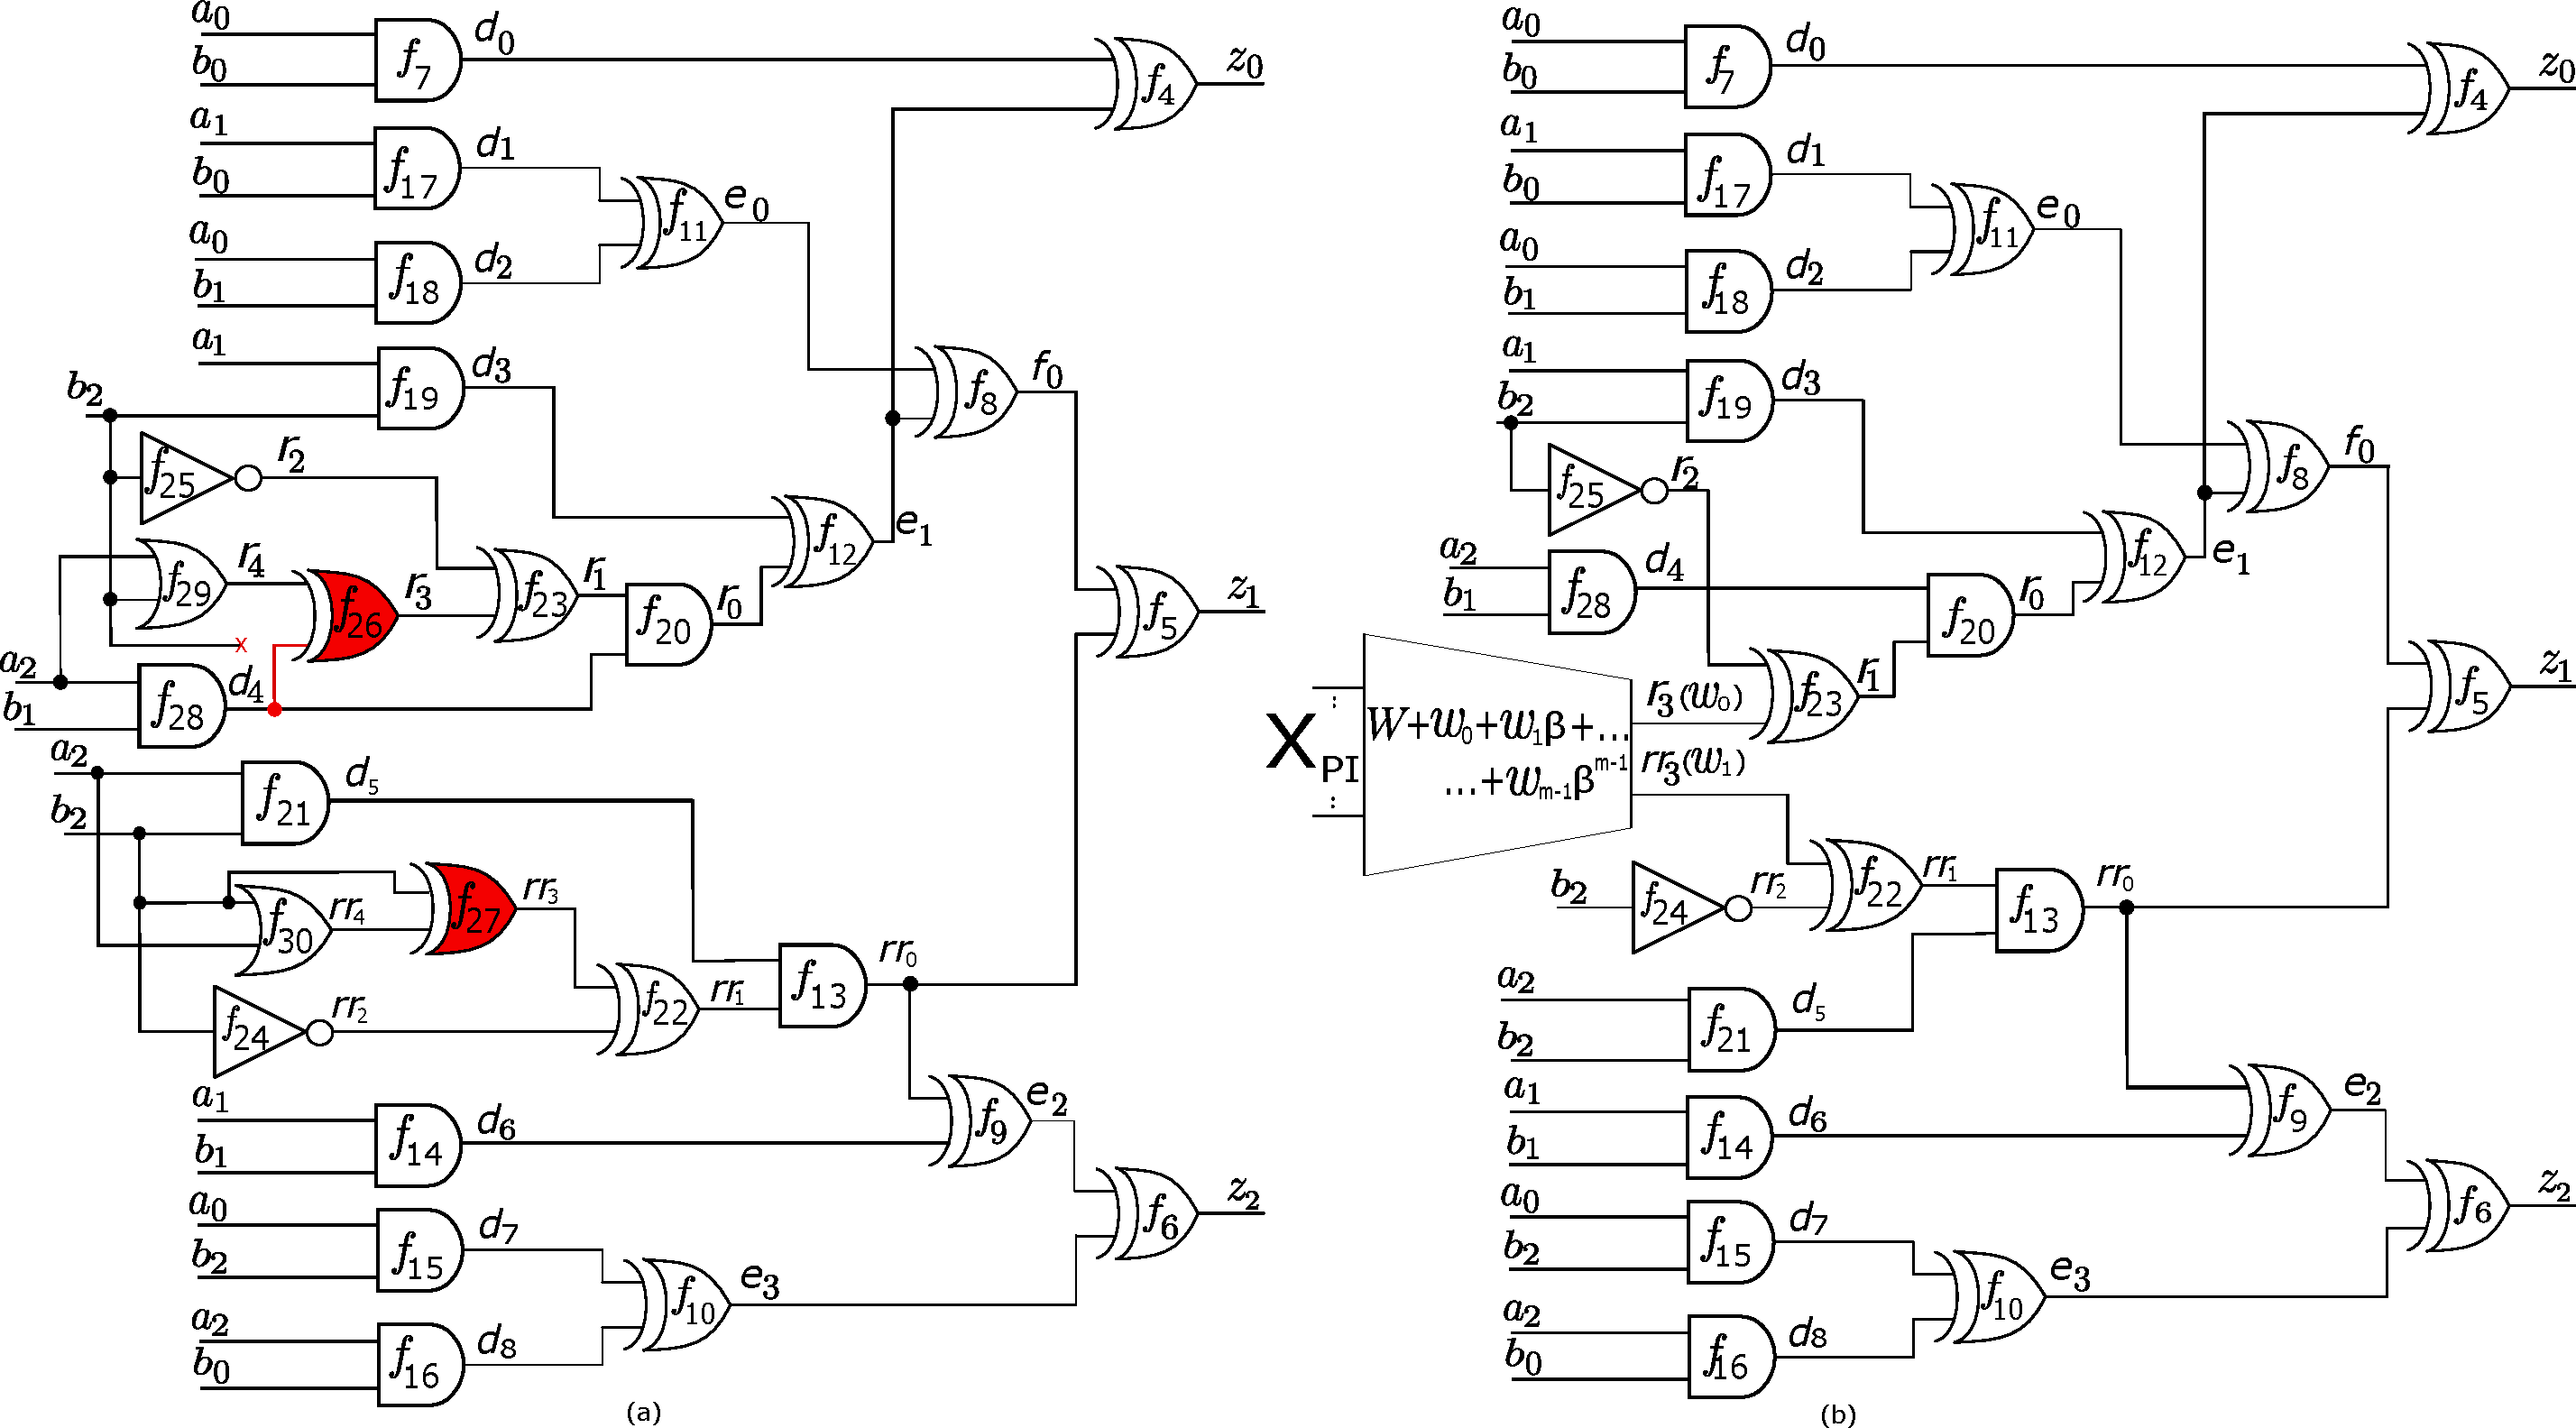
\includegraphics[scale = 0.34]{mas_3_ddc_mfr.pdf}
    \end{center}
    \caption{  
    (a) An incorrect implementation of a circuit $C$: a 3-bit finite
        field multiplier ($n$=3) with bugs introduced at net $r_3$
        (AND gate replaced with an XOR gate and one of the inputs
        misconnected to $d_4$ instead of $b_2$) and net $rr_3$ (AND 
        gate replaced with an XOR gate). (b) The patch function is modeled as a
        2-bit-vector word ($m$=2), $f_W: W+r_3+\be \cdot rr_3$.
        Here, the rectification targets are $W=\{w_0,w_1\}$, where
        $w_0=r_3, w_1=rr_3$).}  
    \label{fig:mas_bug_W}
\end{figure*}

% Rectification begins after verification detects the presence of bugs
% in the design. 
% For verification of finite field arithmetic circuits,
% the approach based on \cite{lv:tcad2013} has been shown to be 
% successful. As the algebraic setup for verification is augmented
% for subsequent rectification, we review the main concepts from
% \cite{lv:tcad2013} below. 
% The algebraic setup used in our MFR checking procedure 
% We perform verification using the approach presented in~\cite{lv:tcad2013}. 
% , utilize the same setup as a starting point for MFR checking. 
% We review the main concepts from~\cite{lv:tcad2013} below:

% We use an augmentation of the algebraic setup presented in~\cite{lv:tcad2013}
% as a starting point for the MFR checking procedure. We therefore review the 
% main concepts and verification setup from~\cite{lv:tcad2013} below:

A multivariate polynomial $f$ over $\Fkn$ is given as a specification,
where $n$ is the operand word-length (datapath size). A corresponding
combinational circuit $C$ is given as its implementation. 
The function implemented by $C$ is modeled with a system of
polynomials over  $R=\Fkn[Z,A,x_1,\dots,x_d]$. Here $\{x_1, \dots,
x_d\}$ correspond to all the bit-level variables (nets) in the
circuit, and $Z,A$ the output and input words, respectively.  The
field $\Fkn$ is constructed as $\Fkn = \Ftwo[X]\pmod{P_n(X)}$, where
$P_n(X)$ is the given primitive polynomial of degree $n$
with $\ga$ as a root (PE), i.e. $P_n(\ga) =0$. 
As $C$ comprises Boolean logic gates, the gates are represented by
polynomials $\pmod{2}$, i.e. over $\F_2 (\subset \Fkn)$, as the
$\B\mapsto \F_2$ mapping:
% as follows: 
\begin{equation}
\label{bool2poly}
\begin{split}
z &=  \neg a \mapsto z+a+1\\
z &=  a \wedge b \mapsto z+a \cdot b\\
z &=  a \vee b \mapsto z+a+b+a \cdot b\\
z &=  a \oplus b \mapsto z+a+b
\end{split}
\end{equation}

% \begin{small} 
% \begin{equation}
% \label{bool2poly}
% \begin{split}
% z =  \neg a &\rightarrow z+a+1 \pmod 2  \\
% z =  a \wedge b &\rightarrow z+a \cdot b \pmod 2\\
% z =  a \vee b &\rightarrow z+a+b+a \cdot b \pmod 2 \\
% z =  a \oplus b &\rightarrow z+a+b \pmod 2 
% \end{split}
% \end{equation}
% \end{small}

Similarly, the primary output and input bits $z_i, a_i: i=0,\dots,n-1$ 
can be correlated to the corresponding operand words $Z,A$ as follows:
\begin{equation}
\label{ip-word-level}
\begin{split}
 f_1: Z + z_0 +\gamma \cdot  z_1 + \dots +\gamma^{n-1} \cdot z_{n-1}\\
 f_2: A + a_0 +\gamma \cdot a_1 + \dots +\gamma^{n-1} \cdot a_{n-1}
\end{split}
\end{equation}

% where $\gamma$ is a PE of $\Fkn$. 
Thus, the circuit is represented
by a set of polynomials $F=\{f_1,\dots,f_s\} \subset
R$. Let $J =\langle F\rangle$ be the ideal
generated by this set.
%Let $X_{PI} \subset \{x_1,\dots,x_d\}$ be the primary input variables
%of the circuit. Let $F_0^{PI}=\{x_i^2-x_i:x_i\in X_{PI}\}$ denote the
%set of bit-level vanishing polynomials in primary inputs, and let $J_0
%= \langle F_0^{PI} \rangle$ be the ideal of vanishing polynomials.
Let $F_0 = \{x_i^2-x_i, Y^{2^n}-Y: x_i \in \text{bit-level variables},
Y \in \text{word-level variables}\}$ be the set of all vanishing
polynomials, and $J_0 = \langle F_0\rangle$ be the corresponding ideal
of all bit- and word-level vanishing polynomials. Then the ideal
$J+J_0 = \langle F \cup F_0\rangle$ models the functionality of
$\impl ~C$.

%% While it is assumed that the given circuit $C$ is buggy, it is important 
%% to note that the verification test can be formulated as {\textit{ideal
%% membership  testing}} of $f$ in $J+J_0$ using
%% GB~\cite{lv:tcad2013}, i.e. by  
%% checking if $f\xrightarrow{GB(J+J_0)}_+0$.
%% It has now become standard practice to impose {\it Reverse Topological Term Order (RTTO)} to 
%% overcome the complexity of GB computations, which ensures the set of
%% polynomials $F\cup F_0$ itself constitute a GB of $J+J_0$. This simplifies
%% the above {\textit{ideal membership testing}} to that of checking if the polynomial division
%% $f\xrightarrow{F+F_{0}}_+0$.

% . When $C$ correctly implements $f$, then $f$ agrees
% with every evaluation of all the nets in $C$. In other words, $f$
% vanishes on $V(J)$, or equivalent{}ly $f \in I(V(J))$. The Strong
% Nullstellensatz in finite fields (Thm. \ref{thm:strong-ns}) tells us
% %Nullstellensatz in finite fields tells us
% that $I(V(J)) = J + J_0$, where $J_0 = \langle F_0 \rangle = \langle x_1^2-x_1,\dots
% ,x_d^2-x_d,Z^{2^n}-Z, A^{2^n}-A\rangle$. Thus, the verification test can be formulated as
% ideal membership testing of $f$ in $J+J_0$ using \Grobner bases: We will
% check if $f\xrightarrow{GB(J+J_0)}_+0$?
% Further, the authors~\cite{lv:tcad2013} impose a specialized term order
% '$>$` called the {\it Reverse Topological Term Order (RTTO)} on the
% polynomials. RTTO is derived by ordering the nets (variables) of $C$
% in reverse topological order from primary outputs to primary inputs,
% and imposing a {\it lex} order on the monomials. It has
% now become standard practice to utilize RTTO-style term orders to 
% overcome the complexity of GB computations.
% RTTO $>$ ensures
% that each net at a gates output appears as a leading term of some
% polynomial in $F$. 
% As each gate output is a distinct net, the
% leading terms of all polynomials in $F$ become relatively
% prime. Thm. 6.1 and Cor. 6.1 in \cite{lv:tcad2013} show that due to
% the above characteristics, {\it RTTO $>$ renders the set of
%   polynomials $F\cup F_0$ itself a GB of $J+J_0$.}
%As the set $F\cup F_0$ is a GB is itself,
% As a result, the expensive GB computation is avoided altogether, and
% the verification check reduces to that of polynomial division
% $f\xrightarrow{F,F_{0}}_+r$, and checking whether $r=0$.
In the manuscript, we use the circuit of Fig. \ref{fig:mas_bug_W} as a
running example to demonstrate our algebraic approach for MFR. 

\begin{Example}
\label{verify_ex}
{\it 
The circuit $C$ in Fig. \ref{fig:mas_bug_W} (a) is an incorrect
implementation of a 3-bit ($n$=3) Mastrovito multiplier. 
The field $\F_{2^3}$ is constructed using $P_3(X)=X^3+X+1$
and let $\ga$ be a PE of $\F_{2^3}$, s.t. $P_3(\ga)=0$. The \spec
~polynomial is $f: Z + A\cdot B$, where $Z$ is the output word, and
$A,B$ the input words. Impose a {\it lex term order} with variable order: 

% \begin{small}
% $\{Z\}>\{A>B\}>\{z_0>z_1>z_2\}>\{d_0>f_0>e_2>e_3\}>\{e_0>e_1>rr_0>d_6>d_7>d_8\}>\{d_1>d_2>d_3>r_0>d_5>rr_1\}>\{r_1>rr_3>rr_2\}>\{r_2>r_3>rr_4\}>\{r_4>d_4\}>\{a_0>a_1>a_2>b_0>b_1>b_2\}$
$\{Z\}>\{A>B\}>\{z_0>z_1>z_2\}>\cdots>\{d_1>d_2>d_3>r_0>d_5>rr_1\}>\{r_1>rr_3>rr_2\}>\{r_2>r_3>rr_4\}>\{r_4>d_4\}>\{a_0>a_1>a_2>b_0>b_1>b_2\}$.
% \end{small}

In this term order, the bit-level variables are ordered
based on the topology of the circuit from POs to PIs, i.e. reverse
topologically. Using this term order, the following polynomials
represent $C$:
%the function implemented by $C$,
%with terms ordered according to RTTO $>$.
% {\small\begin{flalign*}
% f_1:Z + z_0 +\ga z_1 + \ga^2 z_2;  	&\quad f_{16}:d_8 + a_2b_0; \\
% f_2:A + a_0 +\ga a_1 + \ga^2 a_2;  	&\quad f_{17}:d_1 + a_1b_0; \\
% f_3:B + b_0 +\ga b_1 + \ga^2 b_2;  	&\quad f_{18}:d_2 + a_0b_1; \\
% f_4:z_0 + d_0 + e_1;               	&\quad f_{19}:d_3 + a_1b_2; \\
% f_5:z_1 + f_0 + rr_0;             	&\quad f_{20}:r_0 + r_1d_4; \\
% f_6:z_2 + e_2 + e_3;			   	&\quad f_{21}:d_5 + a_2b_2; \\
% f_7:d_0 + a_0b_0;                  	&\quad f_{22}:rr_1 + rr_2+rr_3; \\
% f_8:f_0 + e_0 + e_1;               	&\quad f_{23}:r_1 + r_2+r_3; \\
% f_9:e_2 + rr_0 + d_6;              	&\quad f_{24}:rr_2 + b_2 + 1; \\ 
% f_{10}:e_3 + d_7 + d_8;            	&\quad f_{25}:r_2 + b_2 + 1; \\
% f_{11}:e_0 + d_1 + d_2;      	   	&\quad \red{f_{26}:r_3 + d_4 + r_4;}\\
% f_{12}:e_1 + d_3 + r_0;				&\quad \red{f_{27}:rr_3 + rr_4 + b_2;} \\
% f_{13}:rr_0 + d_5rr_1;			    &\quad f_{28}:d_4 + a_2b_1; \\
% f_{14}:d_6 + a_1b_1;				&\quad f_{29}:r_4 + a_2 + b_2 + a_2b_2; \\
% f_{15}:d_7 + a_0b_2;				&\quad f_{30}:rr_4 + a_2 + b_2 + a_2b_2; \\
% \end{flalign*}}
% \vspace{-0.1in}
% \begin{small}
% \begin{flalign*}
% f_1:Z + z_0 +\ga z_1 + \ga^2 z_2;  	&\quad \dots\\
% f_2:A + a_0 +\ga a_1 + \ga^2 a_2;  	&\quad f_{22}:rr_1 + rr_2+rr_3; \\
% f_3:B + b_0 +\ga b_1 + \ga^2 b_2;  	&\quad f_{23}:r_1 + r_2+r_3; \\
% f_4:z_0 + d_0 + e_1;               	&\quad f_{24}:rr_2 + b_2 + 1; \\ 
% f_5:z_1 + f_0 + rr_0;             	&\quad f_{25}:r_2 + b_2 + 1; \\
% f_6:z_2 + e_2 + e_3;			   	&\quad \red{f_{26}:r_3 + d_4 + r_4;}\\
% f_7:d_0 + a_0b_0;					&\quad \red{f_{27}:rr_3 + rr_4 + b_2;} \\
% f_8:f_0 + e_0 + e_1;				&\quad f_{28}:d_4 + a_2b_1; \\
% f_9:e_2 + rr_0 + d_6;             	&\quad f_{29}:r_4 + a_2 + b_2 + a_2b_2; \\
% \dots								&\quad f_{30}:rr_4 + a_2 + b_2 + a_2b_2;
% \end{flalign*}
% \end{small}
\begin{flalign*}
f_1:Z + z_0 +\ga \cdot z_1 + \ga^2 \cdot z_2;   &\quad f_{22}:rr_1 + rr_3+rr_2; \\
f_2:A + a_0 +\ga \cdot a_1 + \ga^2 \cdot a_2;   &\quad f_{23}:r_1 + r_2+r_3;\\
f_3:B + b_0 +\ga \cdot b_1 + \ga^2 \cdot b_2;   &\quad \red{f_{26}:r_3 + r_4 + d_4;}\\
f_4:z_0 + d_0 + e_1;                &\quad {\red f_{27}:rr_3 + rr_4 + b_2;}\\
f_5:z_1 + f_0 + rr_0;               &\quad \dots\\
\dots                               &\quad f_{30}:rr_4 + a_2+b_2+a_2b_2;
\end{flalign*}

% \vspace{-0.1in}
% \begin{small}
% \begin{flalign*}
% f_1:Z + z_0 +\ga z_1 + \ga^2 z_2;   &\quad f_{22}:rr_1 + rr_2+rr_3; \\
% f_2:A + a_0 +\ga a_1 + \ga^2 a_2;   &\quad f_{23}:r_1 + r_2+r_3; \\
% f_3:B + b_0 +\ga b_1 + \ga^2 b_2;   &\quad \dots\\ 
% f_4:z_0 + d_0 + e_1;                &\quad \red{f_{26}:r_3 + d_4 + r_4;}\\
%                                     &\quad \red{f_{27}:rr_3 + rr_4 + b_2;} \\
%                                     &\quad \dots\\
% \dots                               &\quad f_{30}:rr_4 + a_2 + b_2 + a_2b_2;
% \end{flalign*}
% \end{small}
% The correct circuit will have polynomials $f_{10},f_{12},$ and $f_{18}$ above replaced by 
% $f_{10_c} = e_0 + d_1 + d_2, f_{12_c}:d_5 + a_2b_2,$ and  $f_{18_c}:d_2 + a_2b_1$ respectively.
Then $F = \{f_1,\dots,f_{30}\}$, $F_0 =
\{a_0^2-a_0,\dots,z_2^2-z_2,A^8-A,B^8-B,Z^8-Z\}$. 
%under RTTO $>$, $F\cup F_{0}$ constitutes a GB of
So, ideal $J+J_0=\langle F\cup F_0\rangle$ models $C$. 
% Computing $f: Z + A\cdot  B\xrightarrow{F,F_{0}}_+r$ results in $r =
%  \ga^2(a_1a_2b_1b_2+a_1a_2b_2+a_2b_1b_2) +
%  \ga^1(a_1a_2b_1b_2+a_1a_2b_2) + \ga^0(a_2b_1b_2)$. Since  $r\neq 0$,
%  the circuit is buggy.  
}
\end{Example}
% Our objective now is to identify a set of $m$-target nets where MFR can be
% performed, confirm the existence of a rectification function at these nets, 
% and then to subsequently compute a rectification function. 
%% Note that we can also formulate equivalence
%% verification between a specification $C_s$ and a buggy implementation $C_i$,
%% both given as gate level circuits. The verification problem is modeled as 
%% a word-level miter, with the inputs of $C_s$ and $C_i$ connected together. 
%% Let $Z_{s}$ and $Z_{i}$ represent the word-level outputs of $C_s$ and $C_i$,
%% respectively. With $C_s$ and $C_i$ modeled as polynomial ideals (under RTTO $>$) 
%% $F_s$ and $F_i$, respectively, we formulate the verification problem 
%% as $Z_s-Z_i\xrightarrow{F_s,F_i,F_{0}^{PI}}_+r$, and by checking whether $r=0$?. 
% identifying rectification targets is not clear.
% algorithmically where do you place W? need to formalized and written under net picking W.
% what are the functions that our approach is building?

Since $\F_2 \subset \Fkn$, the polynomials in Eqn. (\ref{bool2poly}) can also 
be interpreted as polynomials over $\Fkn$. The advantage of working
over $\Fkn$ is that we can represent and manipulate both the bit-level 
and $n$-bit word-level polynomials in one unified domain. However, we
are given a patch word-length $m$ which is modeled as an
$m$-bit-vector word over field $\Fkm$.  Since the field $\Fkm$ might
not be compatible with the field $\Fkn$, i.e. $m$ may not divide $n$,
not every $m$-bit-vector can be construed as an element in $\Fkn$. 
To overcome this incompatibility, the following section presents
techniques which enable the modeling of polynomial operations in a
unified domain. 


\section{A Unified Framework for MFR}\label{sec:comps}

%After detecting the presence of bug(s) in the design,
% Having been provided with a set of $m$ targets from $C$, our objective now is to 
% ascertain whether these internal nets admit MFR; i.e. does there exist an $m$-bit patch
% function which rectifies $C$ at these targets? 
% We assume that these targets were provided beforehand or the heuristics 
% proposed in~\cite{SS_Alan:DAC18,SS_Fujita:ISCAS19,SS_Roland:DAC19} were applied to select the same.
%In order to ascertain whether these $m$-targets
%indeed admit MFR, we set up a unified algebraic decision framework as
%follows. 

%\subsection{Word-level Formulation of Patch
%Function}\label{subsec:word_form}
{\it Word-level Rectification Patch:} 
Given a set of $m$-targets, let $W = \{w_0,w_1,\dots,w_{m-1}\}$ denote the $m$-bit vector word,
over which MFR check is to be performed. 
%where the admissibility of the $m$-bit rectification patch is to be
%ascertained.
Here, $w_0,\dots,w_{m-1}\in \{x_1,\dots,x_d\}$
are internal nets of $C$. A rectification patch corresponds to 
a function mapping $f_W: \F_2^{|X_{PI}|}\rightarrow\F_{2^m}$, and
represented as a polynomial function $U(X_{PI}) \in
\F_{2^m}[X_{PI}]$. Here, $U$ is an {\it unknown} polynomial
with variables from $X_{PI}$, and coefficients from $\F_{2^m}$. MFR
then implies that, algebraically, $W = U(X_{PI})$ rectifies the
circuit. 

Such a setup {\it interprets} $U$ as a polynomial function which
evaluates to values in the field $\F_{2^m}$. To construct $\F_{2^m}$,
we {\it select} a degree-$m$ primitive polynomial $P_m(X)\in\F_2[X]$, with
$\beta$ as a root ($P_m(\beta)=0$), such that 
$\F_{2^m} = \F_2[X] \pmod{ P_m(X)}$. Note that any degree-$m$
primitive polynomial ($P_m(X)$) can be selected. This implies that
$\beta$ is a PE of $\F_{2^m}$. Thus, the rectification patch polynomial
function can be represented as: $f_W: W + U(X_{PI}) = W +
\sum_{i=0}^{m-1}\be^iw_i$.  
% \begin{Example}
% \label{target_ex}
% Continuing with our example Ex. \ref{verify_ex}, we analyze the remainder $r$ of verification.
% Note that since the intersection of the fan-in cones of all outputs in $\Oa$ is empty, 
% $C$ doesn't admit single-fix rectification. Further, let $\Ic$ represent the initial cost
% associated with each net in $\In$ assigned based on their respective topological levels from PI.
% Since, each of the nets $\{d_0,e_0,d_2,d_5\}$ lie in the intersection of 2 outputs, we change their 
% cost accordingly.

% {\small
% \begin{flalign*}
% &coefficients(r) = \{ \ga^0,\ga^1,\ga^2\} \implies \Oa = \{z_0,z_1,z_2\} \\
% &\In = \{z_0,z_1,z_2,d_0,f_0,e_2,e_3,e_0,e_1,rr_0,d_6,d_7,d_8,d_1,d_2,d_3,r_0,\\
% &\quad d_5,rr_1,r_1,rr_2,r_2,r_3,rr_3,d_4,r_4,rr_4\} \\
% &\Ic = \{7,7,7,6,6,6,6,5,3,3,5,5,5,4,4,2,2,2,2,1,1,0,0,0,\\
% &\quad -1,-1,-1\} 
% \end{flalign*}
% }
% We partition the set $\Oa$ into 2 ($m$) distinct non-empty subsets
% and compute the corresponding intersection covers. Any individual
% combination of nets from these subsets will always cover the set $\Oa$. 
% {\small
% \begin{flalign*}
% &\Oa = \{\{z_0,z_1\},\{z_2\}\} \\
% &\M = \{\M_0:\{r_4,d_4,r_3,r_2,r_1,r_0,d_3,e_1\},\\
% &\quad\M_1:\{rr_4,rr_3,rr_2,rr_1,d_5,rr_0,d_6,d_7,d_8,e_2,e_3,z_2\}\}
% \end{flalign*}
% }

% We will pick net $r_3$ from $\M_0$ as the first target ($w_0=r_3$) and $rr_3$ 
% from $\M_1$ as the second target ($w_1=rr_3$). The multi-fix patch
% will be modeled as a $2$-bit operand over ${\mathbb{F}}_{2^2}$ constructed as 
% $\Ftwo[X]\pmod{P_2(X)}$ with $\be$ as one of its root, i.e. $P_2(\be)=0$.
% Fig. \ref{fig:mas_bug_W}(b) illustrates $W$ representing the word-level 
% patch as a function of nets $r_3$ and $rr_3$,$ f_w: W+r_3+\be \cdot rr_3$. 
% RTTO with modified variable order:
% $\{Z\}>\{A>B\}>\{z_0>z_1>z_2\}>\{d_0>f_0>e_2>e_3\}>\{e_0>e_1>rr_0>d_6>d_7>d_8\}>\{d_1>d_2>d_3>r_0>d_5>rr_1\}>\{r_1>rr_2\}>\{r_2>{\bf{W}}>r_3>rr_3\}>\{d_4>r_4>rr_4\}>\{a_0>a_1>a_2>b_0>b_1>b_2\}.$ 
% \end{Example}

%\subsection{Composite Field Framework}\label{subsec:comp_fwrk}
{\it Composite Field Framework:} The circuit $C$ is modeled over
$\Fkn$ and the rectification patch is modeled over $\Fkm$. However, the \Grobner basis 
computations for MFR can only be performed over a ring with
coefficients from a single field. We select the field $\Fkk$
of $2^k$ elements, where $k$ is the least common multiple of $m$ and
$n$ ($k=LCM(m,n)$). Thus $\Fkk$ corresponds to the smallest field
containing both $\F_{2^m}$ and $\F_{2^n}$.
% , i.e. $\Fkn \subset \Fkk$ and $\Fkm \subset \Fkk$.
% , thereby allowing every $m$-bit and $n$-bit vector word
% to be construed as elements in a single field $\Fkk$.

\par To construct $\Fkk$, we must now identify
a degree-$k$ primitive polynomial $P_{k}(X)\in\F_2[X]$, and a
corresponding primitive element $\alpha$ such that
$P_k(\alpha)=0$. While there may exist many degree-$k$ primitive
polynomials, the selected $P_k(X)$ needs to conform to specific
conditions imposed by the {\it given} $P_n(X)$, and
the {\it selected} $P_m(X)$.

%, such that $P_n(\gamma) =
%P_m(\beta)=0$.
%%%For this purpose, we exploit the concepts of polynomial
%%%factorization in finite fields \cite{factorization_fq:survey}. 

%Further, care
%should be taken while  
%composing the vanishing polynomials: $x_i^2-x_i$ for the bit-level
%variables, $W^{2^m}-W$ for the $m$-bit bit-vectors, and 
%$Z^{2^n}-Z$ for the $n$-bit bit-vectors.

%% To select the primitive polynomial $P_k(X)$, and a corresponding
%% primitive element $\alpha$, we employ the concept of univariate
%% polynomial facorization in finite fields~\cite{factorization_fq:survey}.

%% \begin{Problem}{[Univariate Polynomial Factorization (UPF)]}
%% Given a monic univariate polynomial $f \in \Fq[x]$, where $\Fq$ is
%% any finite field, find a complete factorization $f = f_1^{e_1}\cdot$ 
%% $\dots f_l^{e_l}$, where $f_1,\dots, f_l$ are pairwise
%% distinct monic irreducible polynomials in $\Fq[x]$, and
%% $e_i\in \Z_{\geq 1}$ are positive integers.
%% \end{Problem}

%% Efficient algorithms to obtain such a factorization in finite fields
%% are well-known \cite{factorization_fq:survey}. %\cite{kaltofen:issac97}, 
%and they are implemented in computer algebra and computational number
%theory tools, such as in \cite{DGPS_410} and \cite{ntl}. We employ
% and we employ the implementation of \cite{ntl} to perform the
% aforementioned UPF. 
Given the primitive elements $\beta, \gamma$ of the fields 
$\F_{2^m},\F_{2^n}$, respectively, let $\alpha$ be a PE of $\Fkk$,
such that $\Fkk \supseteq \F_{2^m},\Fkn$. For the desired unified
computational framework, we represent $\beta, \gamma$ in terms
of $\alpha$. As $\alpha \in \Fkk, \alpha^{2^k-1}=1$. Similarly,
$\beta\in \Fkm$ implies that $\beta^{2^{m}-1}=1$, and $\gamma\in\Fkn$
makes $\gamma^{2^n-1}=1$. Equating
$\be^{2^m-1}=\ga^{2^n-1}=\alpha^{2^k-1} = 1$, we obtain:
% This can be achieved as:
\begin{equation}\label{word-level-rep}
\begin{split}
 \be &= \al^{(2^k-1)/(2^m-1)} = \al^{\mu}\\
 \ga &= \al^{(2^k-1)/(2^n-1)} = \al^{\lambda}
 \end{split}
\end{equation}

With this setup, we show that the desired primitive polynomial
$P_k(X)$ for $\F_2(\alpha)$ exists as a degree-$k$ {\bf common factor}
of $P_n(X^{\lambda})$ and $P_m(X^{\mu})$, and it can be found by
performing univariate polynomial factorizations (UPFs) of
$P_n(X^{\lambda})$ and $P_m(X^{\mu})$ in the base field
$\F_2[X]$. Efficient algorithms to perform UPFs in finite fields are
well-known \cite{factorization_fq:survey}, which can be employed for
this purpose. 

%\begin{small}
\begin{Theorem}\label{thm:Pk}
Given primitive polynomials $P_n(X), P_m(X)$ $\in \F_2[X]$ of degrees
$n,m$, respectively, along with $P_n(\gamma)= P_m(\beta)=0$. Let 
$k=LCM(m,n)$ and $\alpha$ be a PE of $\Fkk$, such that
$\beta=\alpha^\mu$ and $\gamma=\alpha^\lambda$, where
$\mu={(2^k-1)/(2^m-1)}$ and $\lambda={(2^k-1)/(2^n-1)}$.
%Obtain UPFs $P_n(X^\lambda)=P_{n_1}^{a_1}(X)\cdot
%P_{n_2}^{a_2}(X)\cdots P_{n_l}^{a_l}(X)$, and
%$P_{m}(X^\mu)=P_{m_1}^{b_1}(X)\cdots P_{m_g}^{b_g}(X)$, in
%$\F_2[X]$. Then there exists a $P_{n_i}(X) \in
%\{P_{n_1}(X),\dots,P_{n_l}(X)\}$ and a $P_{m_j} (X) \in
%\{P_{m_1}(X),\dots,P_{m_g}(X)\}$ such that $P_k(X) = P_{n_i}(X) =
%P_{m_j}(X)$; i.e.
Perform UPF of $P_n(X^{\lambda})$ and $P_m(X^{\mu})$ in $\F_2[X]$. 
Then there exists a polynomial $P_k(X) \in \F_2[X]$ as a common factor
of $P_m(X^\mu)$ and $P_n(X^\lambda)$, such that $P_k(X)$ is a 
degree-$k$ primitive polynomial with $P_{k}(\alpha)=0$.
\end{Theorem}
%\end{small}

\begin{proof}
Since %$\F_2 \subset \Fkn, \Fkm \subset \Fkk$, and
$\alpha$ is given as a PE of $\Fkk$,  the minimal polynomial of
$\alpha$ is a primitive polynomial. Denote it as $P_k(X)$. Then
$P_k(\alpha)=0$, i.e. $\alpha$ is a root of $P_k(X)$. However,
$P_m(\beta)=0 \implies P_m(\alpha^\mu)=0$. So $P_m(X^\mu)$ also has
$\alpha$ as a root. This implies that $P_k(X)$ divides $P_m(X^\mu)$:
$P_k(X) ~| ~ P_m(X^\mu)$. Similarly, $P_k(X) ~|~ P_n(X^\lambda)$. So
$P_k(X)$ is a common factor of both $P_m(X^\mu)$ and
$P_n(X^\lambda)$. Since $P_m(X^{\mu}), P_n(X^{\lambda}) \in \F_2[X]$,
and their UPFs are also performed in $\F_2[X]$, $P_k(X) \in
\F_2[X]$. Moreover, as $\alpha$ is a PE of $\Fkk$, and $P_k(X)$ is the
minimal polynomial of $\alpha$, we have that $P_k(X)$ is a primitive
polynomial as $\Fkk = \F_2(\alpha)$. Furthermore, by definition, as
the minimal polynomial of $\alpha$, $P_k(X)$ has degree
$=k$. This completes the proof. 
\end{proof}
% The polynomial $P_k(X)$ obtained from Thm. \ref{thm:Pk} can be used to
% construct field $\Fkk = \F_2[X] \pmod{ P_k(X)}$, which encompasses the
% fields corresponding to the circuit ($\Fkn$) and the patch
% ($\Fkm$). Moreover, their respective PE's $\beta, \gamma$, can also be
% related to the PE $\alpha$ of $\Fkk$ by means of
% Eqn. (\ref{word-level-rep}). 


\begin{Example}
\label{composite_ex}
{\it 
Continuing with our rectification example of Fig. \ref{fig:mas_bug_W},
assume that we are given $m=2$ targets: $w_0=r_3$, and $w_1=rr_3$.
The multi-fix patch is modeled as a $2$-bit
operand over $\F_{2^2}=\Ftwo[X]\pmod{P_2(X)=X^2+X+1}$ with
$P_2(\be)=0$. It is given that the 3-bit circuit ($n=3$) is designed
over {\small $\F_{2^3}=\F_2[X]\pmod{P_3(X)=X^3+X+1}$}.  
%Note that we selected $P_2(X)=X^2+X+1$ since that is the only
%primitive polynomial of degree 2. 
With $k=LCM(m,n)=6$, $P_6(X)$ is computed as follows:

Using Eqn. (\ref{word-level-rep}), we have $\gamma=\alpha^9,\beta=\alpha^{21}$. Perform UPFs:
% \begin{multline*}
% 	P_3(X^9) = (X^9)^3+(X^9)+1 =
%   (X^6+X^5+1)(X^6+X^5+X^2+X+1)\\(X^6+X^4+X^3+X+1)(X^6+X^4+X^2+X+1)(X^3+X+1);\\
% 	P_2(X^{21}) = (X^{21})^2+(X^{21})+1 =
%   (X^6+X^5+1)(X^6+X^5+X^2+X+1)\\(X^6+X^4+X^3+X+1)(X^6+X^5+X^3+X^2+1)\\
%   (X^6+X^5+X^4+X+1)(X^6+X+1)(X^6+X^3+1);
% \end{multline*}
\bi
\item ${\scriptstyle P_3(X^9) = (X^9)^3+(X^9)+1 =
  (X^6+X^5+X^2+X+1)(X^6+X^5+1)}$\\${\scriptstyle(X^6+X^4+X^3+X+1)(X^6+X^4+X^2+X+1)(X^3+X+1);}$
\item ${\scriptstyle P_2(X^{21}) = (X^{21})^2+(X^{21})+1 =
  (X^6+X^5+X^2+X+1)}$\\${\scriptstyle (X^6+X^5+1)(X^6+X^4+X^3+X+1)(X^6+X^5+X^3+X^2+1)
  }$\\${\scriptstyle(X^6+X^5+X^4+X+1)(X^6+X+1)(X^6+X^3+1);}$
\ei

Among the degree-6 common factors of ${\scriptstyle P_3(X^9)}$ and
${\scriptstyle P_2(X^{21})}$,  ${\scriptstyle X^6+X^5+X^2+X+1}$ is omitted
since it is non-primitive.  We choose ${\scriptstyle P_6(X) =
  X^6+X^5+1}$ as the required $P_k(X)$. 

Note that if we (incorrectly) choose ${\scriptstyle P_6(X)=X^6 + X^3 +1}$, then it
implies that for its root $\alpha$, we have:
\begin{align*}
\alpha^6 + \alpha^3 + 1 &= 0\\
 (\alpha^3)(\alpha^6 +\alpha^3 + 1) &= 0 ~(\text{multiply by}~\alpha^3)\\
\alpha^9 + \alpha^6 + \alpha^3 &= 0 \\
 \gamma + 1 &= 0
\stepcounter{equation}\tag{\theequation}\label{ll} 
\end{align*}

as $\alpha^9 = \gamma$ and $(\alpha^6 + \alpha^3) = 1$. However,
$\gamma \neq 1$, as $\gamma$ is a PE of $\Fkn$. Therefore, selecting
$P_k(X)$ that does not conform to Thm. \ref{thm:Pk} would lead to
erroneous results.
}
\end{Example}

\section{Word-Level Rectification Check}\label{sec:rcheck}


%% Once the field $\Fkk$, its primitive polynomial $P_k(X)$ and the PE
%% $\alpha$ is identified, we begin the task of formulating the
%% MFR check over $\Fkk$.
% We now show how rectifiability of $C$ against its $\spec$ at
% $m$-distinct target nets $\{w_0,\dots,w_{m-1}\}$ can be ascertained
% (algebraically) at the word-level. 
The $m$-bit target word $W$ is interpreted as an element in $\Fkm$,
such that $W = w_0 + \beta \cdot w_1 + \dots + \beta^{m-1} \cdot
w_{m-1}$,   
% \vspace{-0.2in}
% \begin{align}\label{bit-to-word}
% W = w_0 + w_1\beta + \dots + w_{m-1}\beta^{m-1}
% \end{align}
% \vspace{-0.2in}
where $\beta$ is a PE of $\Fkm$. As $w_0,\dots,w_{m-1}$ are bit-level variables, we first
represent each $w_i$ as a polynomial in terms of the word $W$, and
then substitute their word-level expressions in generators of the
ideal $J+J_0$. 

\begin{Lemma}[From \cite{galois_field:mceliece}]
  \label{lemma:exponent}
Let $\theta_1,\dots,\theta_t \in \Fkm$. Then $(\theta_1+\theta_2+\dots+\theta_t)^{2^i} =
\theta_1^{2^i}+\theta_2^{2^i}+\dots+\theta_t^{2^i}$, for $i\geq 1$.
\end{Lemma}
By virtue of Lemma~\ref{lemma:exponent} and using the relation $W = \sum_{i=0}^{m-1}\beta^i \cdot w_i$, 
we compute $W^{2^j}, 0\leq j < m$: 
\begin{eqnarray}\label{eqn:exponent}
  \begin{aligned}
    W & = w_0 + \dots + \beta^{m-1} \cdot w_{m-1}\\
    W^2 & = w_0^2 + \dots + \beta^{2(m-1)}\cdot w_{m-1}^2\\
    W^2 & = w_0 + \dots + \beta^{2(m-1)} \cdot w_{m-1}
    ~(w_i^2=w_i)\\
    & \dots \\
    W^{2^{m-1}} & = w_0 + \dots + \beta^{2^{m-1}(m-1)}\cdot w_{m-1}
  \end{aligned}
\end{eqnarray}

Considering $w_0,\dots,w_{m-1}$ as $m$ unknowns, and $W$ and $\beta$
as constants, we solve (using Gaussian elimination) the
$m$ linear equations of Eqn. (\ref{eqn:exponent}) to obtain each $w_i$
% $m$ linear equations of~\eqref{eqn:exponent} to obtain each $w_i$
as a polynomial function in $W, \beta$: $w_i =
\mathcal{F}_i(W,\beta)$. Each occurrence of $w_i$ in the generators of
$J+J_0$ can then be replaced with $\mathcal{F}_i(W,\beta)$. 

%\subsection{Rectification Setup}\label{sec:rsetup}
{\it Rectification setup:} Using the aforementioned concepts, the
rectification check is setup in $\Fkk$ as follows: 

\begin{enumerate}
\item Setup the polynomial ring as: $R'=\Fkk[x_1,..,x_d,Z,A$ $,W]$,
  by including the variable $W$, and constructing $\Fkk$ using $P_k(X)$
  (From Thm. \ref{thm:Pk}), with $P_k(\alpha)=0$. 
\item 
  {\it Term order:} Derive a {\it variable order} on the nets of $C$
  such that each variable corresponding to the output of a gate
  appears earlier (lower index) than its immediate inputs. Moreover,
  include the word-level patch variable $W$ in the variable order such
  that $W$ is placed before the target net $w_i$ which has the lowest
  index. Using such a variable order, impose a {\it lex} order on
  the monomials. We call the resulting term order the {\it Word-level
    Rectification Term Order (WRTO)} $>_R$.  
\item Correspondingly update the set of polynomials $F$ (describing the
  logic gates of $C$) to $F'$ as follows: i) Begin by setting
  $F'=F$. Remove from $F'$ the polynomials with $w_i$'s as leading
  terms.
  %ii) Remove the polynomials in the transitive fan-in of
  %target $w_i$'s which do not have re-converging fan-outs.
  ii) Substitute for $w_i$'s the word-level polynomials
  $\mathcal{F}_i(W,\beta)$ as  derived from
  Eqn. (\ref{eqn:exponent}). iii) Add the polynomial $f_W: W +
  \sum_{i=0}^{m-1}\beta^{i} \cdot w_i$ to $F'$. iv) Substitute 
  $\beta = \alpha^{\mu}, \gamma=\alpha^{\lambda}$ for the constants
  (Eqn. (\ref{word-level-rep})). Denote ideal $J'=\langle F'\rangle
  \subset R'$.
\item Update the set of vanishing polynomials $F_0$ to $F'_0$ to
  include the vanishing polynomial $W^{2^m}-W$. This restricts $W$ to
  take values from $\Fkm\subseteq\Fkk$. Let $J'_0=\langle F'_0\rangle$.
\end{enumerate}

The rectification check is then formulated by operating on the
ideal $J'+J'_0=\langle F' \cup F'_0\rangle \subseteq R'$.
%It can be shown that the set $F'\cup F'_0$ also constitutes a
%\Grobner basis of $J'+J'_0$ under WRTO $>_R$, as the polynomials of
%$F'\cup F'_0$ satisfy the same conditions of Thm. 6.1 of
%\cite{lv:tcad2013}.
% The polynomial $f_W$ with leading term $W$ is relatively prime with
% respect to the polynomials representing the other gates.

\begin{Example}
  \label{ex:rect_setup}
% We illustrate how the premise of verification (Example \ref{verify_ex}
% and Fig.~\ref{fig:mas_bug_W}(a)) is modified to 
% setup word-level MFR, depicted in Fig. \ref{fig:mas_bug_W}(b).
{\it 
Continuing with the running example of Fig. \ref{fig:mas_bug_W}(b), 
let the target nets be $W = \{r_3,rr_3\}$, represented by the
polynomial $f_W:W+r_3+\be \cdot rr_3$. We begin with the set $F'=F$,
and derive WRTO to be {\it lex} with variable order: 

% {\bf Vikas:
%   please check if the term order follows reverse topological ordering!}.
  %$\{Z\}>\{A>B\}>\{z_0>z_1>z_2\}>\{d_0>f_0>e_2>e_3\}>\{e_0>e_1>rr_0>d_6>d_7>d_8\}>\{d_1>d_2>d_3>r_0>d_5>rr_1\} >\{r_1>rr_2\}>\{r_2>\bm{W>r_3>rr_3}\}>\{d_4>r_4>rr_4\}>\{a_0>a_1>a_2>b_0>b_1>b_2\}.$
% $\{Z\}>\{A>B\}>\{z_0>z_1>z_2\}>\{d_0>f_0>e_2>e_3\}>\{e_0>e_1>rr_0>d_6>d_7>d_8\}>\{d_1>d_2>d_3>r_0>d_5>rr_1\}>
% \{r_1\}>{\bf \{W\}}>\{rr_3>rr_2\}>\{r_2>r_3>rr_4\}>\{r_4>d_4\}>\{a_0>a_1>a_2>b_0>b_1>b_2\}$.
$\{Z\}>\{A>B\}>\{z_0>z_1>z_2\}>\cdots>\{d_1>d_2>d_3>r_0>d_5>rr_1\}>
\{r_1\}>{\bf \{W\}}>\{{\bf rr_3}>rr_2\}>\{r_2>{\bf r_3}>rr_4\}>\{r_4>d_4\}>\{a_0>a_1>a_2>b_0>b_1>b_2\}$.

The polynomials $f_{26}, f_{27}$ are removed from $F'$, as they
correspond to the target net. Polynomials $f_{22}, f_{23}$ are 
updated to $f'_{22}, f'_{23}$ to represent $rr_3, r_3$ in terms of
$W$. We use Eqn.~(\ref{eqn:exponent}) to represent these bit-level
targets in terms of $W: rr_3=$ $ W^2+W$, and $r_3 = \be W^2 +\be^2
W$. These polynomials are updated as given below:
\begin{align*}
&f'_{22}:rr_1  + (W^2+W) + rr_2\\
&f'_{23}:r_1 + r_2 + (\be W^2 +\be^2 W)\\
&f_W:W + r_3 + \be \cdot rr_3\\     
&\be=\al^{21} \text{ and } \ga=\al^9 \\
&F'=\{f_1,\dots,f_{21},~f'_{22},f'_{23},f_W,\dots,f_{30}\}-\{f_{26},f_{27}\}
\end{align*}
}
\end{Example}
%\vspace{-0.2in}
%\subsection{Rectification Check}
%MFR at target $W$ implies that \underline{there exists} a
%  polynomial function $U(X_{PI})$ which, when implemented at $W$,
%  ensures that the $C$ would implement $f$.
%% Note that
%% $U(X_{PI})$ represents the unresolved polynomial function $\sum_{i=0}^{m-1}\be^iw_i$, 
%% where each net $w_i$ represents a function of the type 
%% %correction$\F_{2^{m}}^{|X_{PI}|}\rightarrow\F_2$.
%% $\F_{2}^{|X_{PI}|}\rightarrow\F_2$.
% {\it Rectification Check:} With the aforementioned MFR setup over
% $\Fkk$ (with $\beta = \alpha^{\mu}, \gamma=\alpha^{\lambda}$), 
We now state the {\it multi-fix rectification theorem} that checks
for the existence of $W = U(X_{PI})$ as a MFR function.

\begin{Theorem}{[Multi-fix Rectification Theorem]}\label{Thm:rect}

Given the specification polynomial $f$, and the implementation
$C$ represented using the ideal $J' = \langle F'\rangle\subset R'$,
where $F'=\{f_1,\dots,\bm{f_W:W+\sum_{i=0}^{m-1}\beta^i \cdot w_i},
\dots,f_s\}$, and $J'_0=\langle F'_0\rangle$ the corresponding ideal
of vanishing polynomials in $R'$. Impose WRTO $>_R$ on $R'$.
%(Setup as described in Sec.\ref{sec:rsetup}),
Construct the following ideals:  
\bi
\item {\small $J'_l = \langle F'_l\rangle =\langle f_1,\dots,f'_W=W+\delta[l],\dots,f_s\rangle$},
  $1 \leq l \leq 2^m$, where $F'_l$ is obtained from $F'$ by
  replacing $f_W \in F'$ with $f'_W: W + \delta[l], 1\leq l \leq 2^m$,
  and $(\delta[1],\dots,\delta[2^{m}]) =
  (0,1,\be,\dots,\be^{2^m-2})$. 
\ei
Reduce $f$ by $F'_l\cup F'_0$ to obtain the remainders $rem_l$: 
$f\xrightarrow{F'_l\cup F'_{0}}_+ rem_l,$  for $1 \leq l \leq 2^m$. 
Then, there exists a polynomial function 
%$U(X_{PI}) = \sum_{i=0}^{m-1}\be^iw_i: \F_{2}^{|X_{PI}|}\rightarrow
%\F_{2^m}$, which, when
$U(X_{PI}): \F_{2}^{|X_{PI}|}\rightarrow \F_{2^m}$, which, when
 implemented at the target $W$, rectifies $C$ to match $f$ \textit{if
   and only if} $\bigcup\limits_{l=1}^{2^m}V(rem_l) = \Ftwo^{|X_{PI}|}$.
% = V(J_{0}^{X_{PI}})$. 
\end{Theorem}

% \begin{table*}[t]
% \footnotesize
% \centering
% \caption{{\footnotesize 
% % The notations in the columns denote the following: 
% Time is in seconds; $\textit{n}$ = Datapath Size, $\textit{m}$ = target word size, 
% $\textit{k}$ = composite field size (degree of $P_k(X)$), 
% AM = Maximum resident memory utilization in Mega Bytes (Average across benchmarks),
% \#G = Number of gates $\times 10^3$, \#BO = Number of incorrect outputs, 
% PBS = Required time for PolyBori setup (ring declaration/poly collection/spec collection),
% % VF = time for verification (Sec.~\ref{sec:verify}), MS = Multi-fix check setup time (Sec.~\ref{sec:comps} [Rectification Setup]), RC = time for MFR check (Thm.~\ref{Thm:rect}), TE = Total execution time.}}
% VMS = Required time for verification, polynomial factorization and computing $P_k(X)$, and MFR setup, 
% RC = Required time for MFR check, TE = Required time for total execution }}
% \label{exptbl}
% \begin{tabular}{!{\vrule width 1pt} c | c | c | c !{\vrule width 1pt} c | c | c | c | c | c !{\vrule width 1pt} c | c | c | c | c | c !{\vrule width 1pt} c | c | c | c | c | c !{\vrule width 1pt}}\noalign{\hrule height 1pt}
% \multicolumn{4}{!{\vrule width 1pt} c !{\vrule width 1pt}}{} & \multicolumn{6}{ c !{\vrule width 1pt}}{Mastrovito} & \multicolumn{6}{ c !{\vrule width 1pt}}{Montgomery} & \multicolumn{6}{ c !{\vrule width 1pt}}{Point Addition}\\ \noalign{\hrule height 1pt}
% {\textit{\textbf{n}}} & {\textit{\textbf{m}}} & {\textit{\textbf{k}}} & {\textbf{AM}} & {\textbf{\#G}} & {\textbf{\#BO}} & {\textbf{PBS}} & {\textbf{VMS}} & {\textbf{RC}} & {\textbf{TE}}& {\textbf{\#G}} & {\textbf{\#BO}} & {\textbf{PBS}} & {\textbf{VMS}} 
% & {\textbf{RC}} & {\textbf{TE}}& {\textbf{\#G}} & {\textbf{\#BO}} & {\textbf{PBS}} & {\textbf{VMS}} & {\textbf{RC}} & {\textbf{TE}}\\ \noalign{\hrule height 1pt}
% %\mb{16}  & \mb{3} & \mb{48}   & 0.03 & Y & 0.8  & 0.04   & 0.02  & 0.01  & 0.10  & 0.9   & 0.1   & 0.2  & 3    & 3.15 & 0.9  & 0.1  & 0.2  & 72    & 74    \\ \hline
% %\mb{32 } & \mb{2} & \mb{32 }  & 0.03 & Y & 2.8  & 0.13   & 0.02  & 0.01  & 0.19  & 2.8   & 0.12  & 0.2  & 0.8  & 1    & 2.9  & 0.17 & 0.2  & 0.98  & 1.2   \\ \hline
% %\mb{48 } & \mb{3} & \mb{48  } & 0.04 & Y & 12.2 & 0.6    & 0.29  & 0.01  & 0.8   & 6.4   & 0.5   & 0.4  & 0.1  & 0.9  & 6.4  & 0.5  & 0.4  & 0.1   & 0.9   \\ \hline
% %\mb{96 } & \mb{7} & \mb{672 } & 1.4  & Y & 24.5 &        &       &       &       & 21    &       &      &      &      & 24.8 &      &      &       &       \\ \hline
% %\mb{16}  & \mb{3} & \mb{48}   & 0.03 & N & 0.8  & 0.04   & 0.02  & 0.02  & 0.11  & 0.9   &       &      &      &      & 0.9  &      &      &       &       \\ \hline
% %\mb{32 } & \mb{7} & \mb{224 } & 0.07 & N & 2.8  &        &       &       &       & 2.8   &       &      &      &      & 2.9  &      &      &       &       \\ \hline
% %\mb{163} & \mb{2} & \mb{326 } & 0.15 & Y & 69.8 & 6.25   &  0.68 & 2.0   & 9.08  & 57.5  & 5.2   & 3.3  & 295   & 305   & 71.6 & 16.1 & 1.9  & 735   & 754   \\ \hline
% \mb{16}  & \mb{5} & \mb{80  } & 100 & 0.8  & 6  & 0.04 & 0.03  & 0.12  & 0.22 & 0.9  & 16  & 0.04 & 0.48 & 35.3     & 35.9 & 0.9  & 7   & 0.06 & 0.08 & 1.73 & 1.9  \\ \hline
% \mb{32 } & \mb{5} & \mb{160 } & 120 & 2.8  & 8  & 0.13 & 0.06  & 0.4   & 0.65 & 2.8  & 32  & 0.13 & 0.54 & 27.6     & 28.3 & 2.9  & 13  & 0.18 & 0.53 & 134  & 135  \\ \hline
% \mb{64 } & \mb{3} & \mb{192 } & 160 & 11.2 & 5  & 0.57 & 0.54  & 227   & 228  & 9.6  & 47  & 0.52 & 0.27 & 1.79     & 2.63 & 10.6 & 64  & 0.84 & 0.45 & 58.1 & 59.5 \\ \hline
% \mb{96 } & \mb{2} & \mb{96  } & 240 & 24.5 & 5  & 1.47 & 0.21  & 0.83  & 2.56 & 21   & 96  & 1.36 & 1.19 & 13.3     & 15.9 & 24.8 & 96  & 2.46 & 0.57 & 14.9 & 18   \\ \hline
% \mb{128} & \mb{2} & \mb{128 } & 370 & 43.2 & 5  & 3.23 & 0.4   & 2.03  & 5.76 & 35.8 & 128 & 2.8  & 1.3  & 64.2     & 68.4 & 43.2 & 128 & 6.45 & 1.55 & 72.8 & 81   \\ \hline
% \mb{163} & \mb{5} & \mb{815 } & 550 & 69.8 & 6  & 6.04 & 1.03  & 11.9  & 21.3 & 57.5 & 128 & 5.19 & 4.34 & 262      & 274  & 71.6 & 22  & 15.7 & 2.31 & 15   & 35.4 \\ \hline
% \mb{233} & \mb{2} & \mb{466 } & 750 & 119  & 3  & 13   & 1     & 0.01  & 14.2 & 112  & 233 & 11.5 & 3.4  & 360      & 375  & 122  & 233 & 19.2 & 1.5  & 0.15 & 21.5 \\ \hline
% \mb{283} & \mb{2} & \mb{566 } & 1300& 190  & 2  & 38   & 1.9   & 0.1   & 42.3 & 171  & 283 & 35   & 9.2  & 1503     & 1549 & 208  & 4   & 80.4 & 4.1  & 0.1  & 86.6 \\ \hline
% \mb{409} & \mb{2} & \mb{818 } & 2400& 384  & 2  & 190  & 3.6   & 0.1   & 195  & 340  & 409 & 134  & 9    & 4920*    & 5064 & 368  & 409 & 220  & 7    & 2007 & 2237 \\ \hline
% \mb{571} & \mb{2} & \mb{1042} & 5000& 827  & 5  & 2150 & 8.9   & 0.1   & 2162 & 663  &     & 1313 & 73   & 0.2$\td$ & 1395 & 813  & 5   & 2583 & 17.7 & 880  & 3490 \\ \hline\hline
% \mb{16}  & \mb{7} & \mb{112 } & 100 & 0.8  & 11 & 0.04 & 0.11  & 4.96  & 5.14 & 0.9  & 13  & 0.05 & 1.54 & 228      & 230  & 0.9  & 12  & 0.05 & 0.62 & 32.9 & 33.6 \\ \hline
% \mb{32 } & \mb{5} & \mb{160 } & 120 & 2.8  & 8  & 0.13 & 0.04  & 0.81  & 1.03 & 2.8  & 32  & 0.13 & 0.95 & 100      & 101  & 2.9  & 13  & 0.18 & 0.71 & 244  & 245  \\ \hline
% \mb{64 } & \mb{3} & \mb{192 } & 160 & 11.2 & 5  & 0.58 & 0.18  & 1.64  & 2.45 & 9.6  & 47  & 0.51 & 0.39 & 10.4     & 11.4 & 10.6 & 5   & 0.79 & 0.25 & 3.96 & 5.05 \\ \hline
% \mb{96 } & \mb{2} & \mb{96  } & 240 & 24.5 & 5  & 1.48 & 0.2   & 0.04  & 1.77 & 21   & 96  & 1.34 & 2.04 & 87.5     & 90.9 & 24.8 & 96  & 2.44 & 0.62 & 35.5 & 38.6 \\ \hline
% \mb{128} & \mb{2} & \mb{128 } & 370 & 43.2 & 5  & 3.21 & 0.43  & 0.1   & 3.84 & 35.8 & 128 & 2.7  & 1.3  & 66       & 70   & 43.2 & 128 & 6.1  & 1    & 73   & 81   \\ \hline
% \mb{163} & \mb{5} & \mb{815 } & 550 & 69.8 & 6  & 6.3  & 1.06  & 12    & 21.7 & 57.5 & 128 & 5.31 & 5.26 & 524      & 537  & 71.6 & 22  & 15.8 & 2.46 & 37   & 57.6 \\ \hline
% \mb{409} & \mb{2} & \mb{818 } & 2400& 384  & 2  & 208  & 3.76  & 0.03  & 212  & 340  & 13  & 127  & 6.76 & 0.13     & 135  & 368  & 3   & 210  & 8.04 & 928  & 1146 \\ \hline
% \mb{571} & \mb{2} & \mb{1042} & 5000& 827  & 5  & 2246 & 8.53  & 0.11  & 2256 & 663  & 427 & 1358 & 62.3 & 2.24     & 1424 & 813  & 5   & 2433 & 16.7 & 4.94 & 2457 \\ \noalign{\hrule height 1pt}
% \end{tabular}
% \end{table*}

\begin{table*}[t]
\caption{ 
% The notations in the columns denote the following: 
Time is in seconds; $\textit{n}$ = Datapath Size, $\textit{m}$ = target word size, 
$\textit{k}$ = composite field size (degree of $P_k(X)$), 
AM = Maximum resident memory utilization in Mega Bytes (Average across benchmarks),
\#G = Number of gates $\times 10^3$, \#BO = Number of incorrect outputs, 
PBS = Required time for PolyBori setup (ring declaration/poly collection/spec collection),
% VF = time for verification (Sec.~\ref{sec:verify}), MS = Multi-fix check setup time (Sec.~\ref{sec:comps} [Rectification Setup]), RC = time for MFR check (Thm.~\ref{Thm:rect}), TE = Total execution time.}}
VMS = Required time for verification, polynomial factorization and computing $P_k(X)$, and MFR setup, 
RC = Required time for MFR check, TE = Required time for total execution }

\label{exptbl}
\resizebox{\linewidth}{!}{
\begin{tabular}{!{\vrule width 1pt} c | c | c | c !{\vrule width 1pt} c | c | c | c | c | c !{\vrule width 1pt} c | c | c | c | c | c !{\vrule width 1pt} c | c | c | c | c | c !{\vrule width 1pt}}\noalign{\hrule height 1pt}
\multicolumn{4}{!{\vrule width 1pt} c !{\vrule width 1pt}}{} & \multicolumn{6}{ c !{\vrule width 1pt}}{Mastrovito} & \multicolumn{6}{ c !{\vrule width 1pt}}{Montgomery} & \multicolumn{6}{ c !{\vrule width 1pt}}{Point Addition}\\ \noalign{\hrule height 1pt}

{\textit{\textbf{n}}} & {\textit{\textbf{m}}} & {\textit{\textbf{k}}} & {\textbf{AM}} & {\textbf{\#G}} & {\textbf{\#BO}} & {\textbf{PBS}} & {\textbf{VMS}} & {\textbf{RC}} & {\textbf{TE}}& {\textbf{\#G}} & {\textbf{\#BO}} & {\textbf{PBS}} & {\textbf{VMS}} 
& {\textbf{RC}} & {\textbf{TE}}& {\textbf{\#G}} & {\textbf{\#BO}} & {\textbf{PBS}} & {\textbf{VMS}} & {\textbf{RC}} & {\textbf{TE}}\\ \noalign{\hrule height 1pt}

%\mb{16}  & \mb{3} & \mb{48}   & 0.03 & Y & 0.8  & 0.04   & 0.02  & 0.01  & 0.10  & 0.9   & 0.1   & 0.2  & 3    & 3.15 & 0.9  & 0.1  & 0.2  & 72    & 74    \\ \hline
%\mb{32 } & \mb{2} & \mb{32 }  & 0.03 & Y & 2.8  & 0.13   & 0.02  & 0.01  & 0.19  & 2.8   & 0.12  & 0.2  & 0.8  & 1    & 2.9  & 0.17 & 0.2  & 0.98  & 1.2   \\ \hline
%\mb{48 } & \mb{3} & \mb{48  } & 0.04 & Y & 12.2 & 0.6    & 0.29  & 0.01  & 0.8   & 6.4   & 0.5   & 0.4  & 0.1  & 0.9  & 6.4  & 0.5  & 0.4  & 0.1   & 0.9   \\ \hline
%\mb{96 } & \mb{7} & \mb{672 } & 1.4  & Y & 24.5 &        &       &       &       & 21    &       &      &      &      & 24.8 &      &      &       &       \\ \hline
%\mb{16}  & \mb{3} & \mb{48}   & 0.03 & N & 0.8  & 0.04   & 0.02  & 0.02  & 0.11  & 0.9   &       &      &      &      & 0.9  &      &      &       &       \\ \hline
%\mb{32 } & \mb{7} & \mb{224 } & 0.07 & N & 2.8  &        &       &       &       & 2.8   &       &      &      &      & 2.9  &      &      &       &       \\ \hline
%\mb{163} & \mb{2} & \mb{326 } & 0.15 & Y & 69.8 & 6.25   &  0.68 & 2.0   & 9.08  & 57.5  & 5.2   & 3.3  & 295   & 305   & 71.6 & 16.1 & 1.9  & 735   & 754   \\ \hline
\mb{16}  & \mb{5} & \mb{80  } & 100 & 0.8  & 6  & 0.04 & 0.03  & 0.12  & 0.22 & 0.9  & 16  & 0.04 & 0.48 & 35.3     & 35.9 & 0.9  & 7   & 0.06 & 0.08 & 1.73 & 1.9  \\ \hline
\mb{32 } & \mb{5} & \mb{160 } & 120 & 2.8  & 8  & 0.13 & 0.06  & 0.4   & 0.65 & 2.8  & 32  & 0.13 & 0.54 & 27.6     & 28.3 & 2.9  & 13  & 0.18 & 0.53 & 134  & 135  \\ \hline
\mb{64 } & \mb{3} & \mb{192 } & 160 & 11.2 & 5  & 0.57 & 0.54  & 227   & 228  & 9.6  & 47  & 0.52 & 0.27 & 1.79     & 2.63 & 10.6 & 64  & 0.84 & 0.45 & 58.1 & 59.5 \\ \hline
\mb{96 } & \mb{2} & \mb{96  } & 240 & 24.5 & 5  & 1.47 & 0.21  & 0.83  & 2.56 & 21   & 96  & 1.36 & 1.19 & 13.3     & 15.9 & 24.8 & 96  & 2.46 & 0.57 & 14.9 & 18   \\ \hline
\mb{128} & \mb{2} & \mb{128 } & 370 & 43.2 & 5  & 3.23 & 0.4   & 2.03  & 5.76 & 35.8 & 128 & 2.8  & 1.3  & 64.2     & 68.4 & 43.2 & 128 & 6.45 & 1.55 & 72.8 & 81   \\ \hline
\mb{163} & \mb{5} & \mb{815 } & 550 & 69.8 & 6  & 6.04 & 1.03  & 11.9  & 21.3 & 57.5 & 128 & 5.19 & 4.34 & 262      & 274  & 71.6 & 22  & 15.7 & 2.31 & 15   & 35.4 \\ \hline
\mb{233} & \mb{2} & \mb{466 } & 750 & 119  & 3  & 13   & 1     & 0.01  & 14.2 & 112  & 233 & 11.5 & 3.4  & 360      & 375  & 122  & 233 & 19.2 & 1.5  & 0.15 & 21.5 \\ \hline
\mb{283} & \mb{2} & \mb{566 } & 1300& 190  & 2  & 38   & 1.9   & 0.1   & 42.3 & 171  & 283 & 35   & 9.2  & 1503     & 1549 & 208  & 4   & 80.4 & 4.1  & 0.1  & 86.6 \\ \hline
\mb{409} & \mb{2} & \mb{818 } & 2400& 384  & 2  & 190  & 3.6   & 0.1   & 195  & 340  & 409 & 134  & 9    & 4920*    & 5064 & 368  & 409 & 220  & 7    & 2007 & 2237 \\ \hline
\mb{571} & \mb{2} & \mb{1042} & 5000& 827  & 5  & 2150 & 8.9   & 0.1   & 2162 & 663  &     & 1313 & 73   & 0.2$\td$ & 1395 & 813  & 5   & 2583 & 17.7 & 880  & 3490 \\ \hline\hline
\mb{16}  & \mb{7} & \mb{112 } & 100 & 0.8  & 11 & 0.04 & 0.11  & 4.96  & 5.14 & 0.9  & 13  & 0.05 & 1.54 & 228      & 230  & 0.9  & 12  & 0.05 & 0.62 & 32.9 & 33.6 \\ \hline
\mb{32 } & \mb{5} & \mb{160 } & 120 & 2.8  & 8  & 0.13 & 0.04  & 0.81  & 1.03 & 2.8  & 32  & 0.13 & 0.95 & 100      & 101  & 2.9  & 13  & 0.18 & 0.71 & 244  & 245  \\ \hline
\mb{64 } & \mb{3} & \mb{192 } & 160 & 11.2 & 5  & 0.58 & 0.18  & 1.64  & 2.45 & 9.6  & 47  & 0.51 & 0.39 & 10.4     & 11.4 & 10.6 & 5   & 0.79 & 0.25 & 3.96 & 5.05 \\ \hline
\mb{96 } & \mb{2} & \mb{96  } & 240 & 24.5 & 5  & 1.48 & 0.2   & 0.04  & 1.77 & 21   & 96  & 1.34 & 2.04 & 87.5     & 90.9 & 24.8 & 96  & 2.44 & 0.62 & 35.5 & 38.6 \\ \hline
\mb{128} & \mb{2} & \mb{128 } & 370 & 43.2 & 5  & 3.21 & 0.43  & 0.1   & 3.84 & 35.8 & 128 & 2.7  & 1.3  & 66       & 70   & 43.2 & 128 & 6.1  & 1    & 73   & 81   \\ \hline
\mb{163} & \mb{5} & \mb{815 } & 550 & 69.8 & 6  & 6.3  & 1.06  & 12    & 21.7 & 57.5 & 128 & 5.31 & 5.26 & 524      & 537  & 71.6 & 22  & 15.8 & 2.46 & 37   & 57.6 \\ \hline
\mb{409} & \mb{2} & \mb{818 } & 2400& 384  & 2  & 208  & 3.76  & 0.03  & 212  & 340  & 13  & 127  & 6.76 & 0.13     & 135  & 368  & 3   & 210  & 8.04 & 928  & 1146 \\ \hline
\mb{571} & \mb{2} & \mb{1042} & 5000& 827  & 5  & 2246 & 8.53  & 0.11  & 2256 & 663  & 427 & 1358 & 62.3 & 2.24     & 1424 & 813  & 5   & 2433 & 16.7 & 4.94 & 2457 \\ \noalign{\hrule height 1pt}
\end{tabular}
}
\end{table*}

%\begin{Proof}
%We omit the proof due to the space limitation. 
%\end{Proof}

A detailed proof of the above theorem can be devised using the
ideal-variety correspondences. However, the proof is omitted due to
the strict page  limit on the manuscript. Instead, we explain the
intuition behind Thm.~\ref{Thm:rect}, and show how it can be applied
for MFR check.

Due to WRTO $>_R$, each $rem_l$ comprises only $X_{PI}$
variables. This is because under WRTO $>_R$, each gate output becomes
a leading term of some polynomial in $F'$. However, as primary inputs 
cannot be gate outputs, they do not appear as a leading term
of any polynomial. As a result, the computation
$f\xrightarrow{F'_l\cup F'_0}_+rem_l$ cancels all non primary input
variables during polyomial division, and results in remainders with
only primary inputs in their support. Hence, $V(rem_l) \subseteq
\F_{2}^{|X_{PI}|}$. The variety of  $rem_l$  corresponds to the set of
assignments to primary inputs $X_{PI}$ (minterms) where the
specification $f$ agrees with the implementation $C$. Thus, the
condition of Thm.~\ref{Thm:rect} implies that the union of individual
varieties of $rem_l$'s comprises the entire input test set. Thus, for
every minterm from the input test space, there exists an assignment
$\delta[l]$ to $W$ where $f$ and $C$ match.  Consequently, there
exists a function $U(X_{PI})$ that can be computed to rectify every
error minterm.  

% \begin{Proof}
% As the correction at target $W$ makes $C$ match $f$, $f$ should vanish on
% $V_{\Fkk}(J')$.
% Moreover, each $rem_l$ comprises only $X_{PI}$ variables. This is
% because WRTO $>_R$ ensures that each non primary input variable (each gate
% output and  word-level variable) appears as the leading term of some
% polynomial in $F'$. Thus each non primary input variable is canceled
% in the reduction $f\xrightarrow{F'_l, F'_{0}}_+ rem_l$. Furthermore,
% as $X_{PI}$ take values in $\F_2$, $x^2=x, \forall x \in
% X_{PI}$. Hence, 
% % even though $V_{\Fkk}(J')$ is evaluated in $\Fkk$,
% $V(rem_l) \subseteq \F_{2}^{|X_{PI}|}$. Thus, the rectification theorem
%  can be equivalently stated as: ``$f$ vanishes on
% \begin{small}
% $V_{\Fkk}(J') \iff \bigcup\limits_{l=1}^{2^m}V(rem_l) = \Ftwo^{|X_{PI}|}$''.
% \end{small} 

% (i) {\bf To prove ``$\Rightarrow$''}: Let $x_{PI} \in \Ftwo^{|X_{PI}|}$ be an
% assignment to the primary input variables of $C$. Every assignment
% $x_{PI}$ results in a corresponding assignment $x_{int}$ 
% to rest of the variables in $C$. For each such point $(x_{PI},x_{int})\in \Fkk$,
% the target $W$ evaluates to one of the values in the list $\delta$,
% i.e. $(0,1,\be,\dots,\beta^{2^m-2})$. When $W = 0$, $J'_1$ vanishes on
% the point $(x_{PI},x_{int})$. Likewise, $J'_2$ vanishes on
% $(x_{PI},x_{int})$ when $W = 1$, and so on. Since
% $f\xrightarrow{F'_l\cup F'_0}_+rem_l,1 \leq l \leq 2^m$, and $f$ vanishes
% on the point $(x_{PI},x_{int})$ to begin with, we obtain that for
% every  primary input assignment $x_{PI}$, one of the $rem_l$ vanishes. This
% implies that $ \bigcup\limits_{l=1}^{2^m}V(rem_l) = \Ftwo^{|X_{PI}|}$.

% (ii) {\bf To prove ``$\Leftarrow$''}: Say there exists an assignment to the
% primary inputs $x_{PI} \in \Ftwo^{|X_{PI}|}$ such that $rem_1$ vanishes on
% $x_{PI}$, i.e. $rem_1(x_{PI})=0$. For the given point $x_{PI}$, the rest of the variables 
% of $C$ get a corresponding assignment $x_{int}$. 
% As $f\xrightarrow{F'_1\cup F'_0}_+ rem_1$, we have that $f$ is a member of the
% ideal $J'_1 + J'_0 + \langle rem_1 \rangle$. Therefore, when
% $rem_1(x_{PI})=0$, the ideal $J'_1$ also vanishes on $(x_{PI},x_{int}) \in \Fkk$
% because the tuple $(x_{PI},x_{int})$ is a valid evaluation of the circuit.
% Further, $J'_0$ by definition vanishes everywhere in $R'$. This implies that
% $f(x_{PI},x_{int})=0$. The argument similarly holds for each
% $rem_{l}$ vanishing on some $x_{PI}$. This proves that for all primary
% inputs, if any $rem_l:1 \leq l \leq 2^m$ vanishes, then $f$ vanishes too; and 
% that completes the proof.
% \end{Proof}
 

%where the union of
%varieties corresponds to the product of ideals and is characterized by
%Strong Nullstellensatz over finite fields ({\red refer Strong
%  Nullstellensatz}). 
%% \begin{small}
%% \begin{align*}
%% &\bigcup\limits_{l=1}^{2^m}V(rem_l) =V_{\Ftwo}( \prod_{l=1}^{2^m}
%%   rem_l)= V_{\Ftwo}( \langle \prod_{l=1}^{2^m} rem_l \rangle +
%%   J_0^{X_{PI}} ) \\
%% & \quad\quad\quad\quad\quad\quad\quad\quad = V_{\Ftwo}(\langle \prod_{l=1}^{2^m} rem_l \rangle+ J_0^{PI})
%%   % V_{\Fqbar}(\langle r_1\cdot \dots r_{2^m} \rangle+ J_0^{PI}) \\
%% \end{align*}
%% \end{small}
%% Thus, to check for MFR at target $W$, we need
%% to check if $\prod_{l=1}^{2^m} rem_l\xrightarrow{J_{0}^{PI}}_+0$?  

Let $J_0^{X_{PI}} = \langle x^2-x: x\in X_{PI}\rangle$. Then
$V(J_0^{X_{PI}}) = \F_2^{|X_{PI}|}$. As the union of varieties
corresponds to the variety of the product of corresponding ideals
(cf. Section \ref{sec:prelim}), we have that: 
$\bigcup\limits_{l=1}^{2^m}V(rem_l) =
%V_{\Ftwo}( \prod_{l=1}^{2^m}rem_l)=
V_{\Ftwo}( \langle \prod_{l=1}^{2^m} rem_l \rangle +
J_0^{X_{PI}} )$.  
Therefore, to check for MFR at target $W$, the test ``Is
${\scriptstyle \bigcup\limits_{l=1}^{2^m}V(rem_l) =
  \F_2^{|X_{PI}|}}$'' can be performed by checking if
$\prod_{l=1}^{2^m} rem_l\xrightarrow{J_{0}^{PI}}_+0$. 

\begin{Example}
\label{ex:3}
{\it 
Continuing on with the example from Ex. \ref{ex:rect_setup}, we
demonstrate the rectification check at $W=\{r_3,rr_3\}$. 

Constructing the $J'_l$ ideals:
\bi
\item {\small$J'_1 = \langle F'_1\rangle$, where $F'_1[f'_W]=W+\delta[1]=W$}
\item {\small$J'_2 = \langle F'_2\rangle$, where $F'_2[f'_W]=W+\delta[2]=W+1$}
\item {\small$J'_3 = \langle F'_3\rangle$, where $F'_3[f'_W]=W+\delta[3]=W+\be=W+\alpha^{21}$}
\item {\small$J'_4 = \langle F'_4\rangle$, where $F'_4[f'_W]=W+\delta[4]=W+\be^2=W+\alpha^{42}$}
\ei
Reducing the $\spec$ $f: Z+A\cdot B$ modulo these ideals, we get:
\bi
\item $rem_1 = f \xrightarrow[]{F'_1\cup F'_{0}}_+{\al^{27} (a_2b_1b_2)+\al^{36} (a_2b_2)}$
\item $rem_2 = f \xrightarrow[]{F'_2\cup F'_{0}}_+{\al^{27} (a_2b_1b_2+a_2b_1)+\al^{36} (a_2b_2)}$
\item $rem_3 = f \xrightarrow[]{F'_3\cup F'_{0}}_+{\al^{27} (a_2b_1b_2)}$
\item $rem_4 = f \xrightarrow[]{F'_4\cup F'_{0}}_+{\al^{27} (a_2b_1b_2+a_2b_1)}$
\ei

When we compute the product $\prod_{l=1}^{4} rem_l$, 
and reduce it by $J_{0}^{X_{PI}}$ in $\F_{2^6}$ with
$P_6(\alpha)=0$, we obtain the remainder 0, thus confirming
that the target $W=\{w_0=r_3,w_1=rr_3\}$ indeed admits correction.
Even though it is beyond the scope of this paper, $W=a_2b_1b_2+\be \cdot a_2b_2$ 
is a polynomial which can be computed to rectify the circuit. 
% In fact, the rectification test also passes with nets $d_2$ and $d_5$;
% implying that we could have selected $w_0$ to be $d_2$ instead of $e_0$. 
% However, the rectification test fails when $w_0=d_0$ and
%  $w_1=d_5$. When the problem is formulated with these nets, $\prod_{l=1}^{4} 
%  rem_l\xrightarrow{J_{0}^{X_{PI}}}_+\al^9a_2b_1b_2+\al^{36}a_2b_2$  implying that
%  these nets do not admit correction.   
}
\end{Example}

% \begin{algorithm}\label{rect_flow_alg}
% \caption{Rectification of finite field arithmetic circuits}\label{pseudocode}
% \begin{algorithmic}[1]
% \Require $\spec:f, buggy~\impl: C$ modeled as a polynomial ideal $F=\{f_1\dots,f_s\}$ under $RTTO >$ 
% \Assume {$C$ doesn't admit single-fix rectification} //~\cite{Vkrao:FMCAD18}
% \Ensure {Rectification of $C$ to match $f$}
% \Procedure{$rectification$}{} 
% \State {remainder = $verify(f,F+F_0)$} // Sec.\ref{sec:verify}
% \State {$\Oa = analyze$(remainder)} //Sec. V.1~\cite{Vkrao:FMCAD18}
% \State {$\In = PotentialNets()$} //Sec.\ref{subsec:target_nets}
% \State {$m = 2$; rectified = $False; \mathcal{O}_A = \emptyset ; F_w = \emptyset$}
% \Do %1
% \State {$\Oa^i = uniquePartition(\Oa,m)$}\label{prtn}
% \If {$\Oa^i \notin \mathcal{O}_A$}
% \State {$\mathcal{O}_A=\mathcal{O}_A \cup \Oa^i$}
% \State {$\M^i = intersectionCover(\Oa^i)$}  
% \State {$f_w=pickTargets(\M^i,m)$}\label{ptrgt}
% \If {$f_w \notin F_w$}
% \State {$F_w=F_w \cup f_w$}
% \State {$MFRSetup()$} //Sec.\ref{subsec:comp_fwrk}
% \If {$MFRCheck(F')==0$} //Sec.\ref{sec:rcheck}
% \State {rectified = $True$}
% \State {patch = $rectFunction$()} //Sec.\ref{sec:rfunc}
% \Else
% \State {$goto~\ref{ptrgt}$}
% \EndIf
% \Else
% \State {$goto~\ref{prtn}$}
% \EndIf
% \Else
% \State $m++$
% \EndIf
% \doWhile {((!rectified) $\&\&$ $m \le |\Oa|$)} %1
% \State \Return patch
% \EndProcedure
% \end{algorithmic}
% \end{algorithm}

\section{Experimental Results}
\label{sec:exp}
% All the algorithms and computations were implemented in Polybori engine~\cite{pbori:JSC09}.
% Our implementation is based on 
% Based on the above discussion, we will: i) model GBR as the
% algebra of unate cube sets; ii) use ZDDs as the implicit
% data-structure for this GBR; and iii) devise efficient implementation
% of GBR by exploiting the special structure imposed by RTTO on the
% ZDD graph.  
% In \cite{Minato:DAC94}, {\it Minato} demonstrated that ZDDs are an
% efficient data-structure for implicit manipulation (algebra) of unate
% cube sets. 
%Since a monomial of a Boolean
%polynomial is a unate cube, we can interpret a Boolean polynomial as a
%set of unate cubes; and each monomial (cube) as a set of
%variables. 
% {\it Minato} has shown (\cite{Minato:DAC93}\cite{Minato:DAC94}) how the set union, intersection and
% difference operations can be performed recursively on the ZDDs, 
% and they have been implemented using the {\it ite-operator (if-then-else)} in
% decision diagrams such as the CUDD \cite{Somenzi:CUDD} package. 
% By analyzing the {structure of ZDDs} for 
% polynomial representation, we show how this 
% GB-reduction can be efficiently implemented using algorithms that
% specifically manipulate the ZDD graph. 

% {\it implicit} characteristic set representation 
% for storing and manipulating polynomials. 
% The same framework 
% is utilized towards implementing incremental rectification check.
% Our implementation utilizes PolyBori’s~\cite{pbori:JSC09} reduction procedure with 
% ZDD~\cite{Minato:DAC93,Minato:DAC94} as the underlying data structure to 
% model the MFR framework. 
% % Our rectification approach operates 
% % over the ring $\ftkwring$, whereas ZDDs can only be used 
% % to represent polynomials and perform reductions in $\ftring$.
% % % We extend these operations to accommodate the sum and product operations
% % % $\pmod{2}$, i.e. polynomial algebra in $\Ftwo[x_1,\dots,x_d]$, by 
% % % manipulating sets of combinations using ZDDs. 
% % However, as the core of our computations is based on a
% % couple of Spoly reductions, it is possible to employ ZDDs
% % ~\cite{Utkarsh:TCAD19}. 
% Taking inspiration from~\cite{Utkarsh:TCAD19}, we make use of the 
% {\it implicit} characteristic set representation 
% for storing and manipulating polynomials. 
% % The same framework 
% % is utilized towards implementing incremental rectification check.
% In addition, we have developed a high level finite field engine
%  to model bit-vector and coefficient computations.
% Further, we have also utilized polynomial algebra tool {\sc Singular}
% ~\cite{DGPS_410} for finding primitive polynomials to help model composite field characteristics.
% Subject to the given variable order, a ZDD represents a 
% Boolean function canonically. Just as with BDDs, every node in a ZDD
% is assigned an index, which corresponds to the variable order imposed
% on the diagram. A detailed description of ZDDs and
% their capabilities for solving logic optimization and sparse
% combinatorial problems can be found in \cite{Minato:DAC93} and
% \cite{Minato:DAC94}. 
% Minato has shown ([94][95]) how the set union, intersection and difference operations
% can be performed recursively on the ZDDs, and they have been implemented using the
% ite-operator (if-then-else) in decision diagrams such as the CUDD [118] package. We extend
% these operations to accommodate the sum and product operations ( mod 2 ) , i.e. polyno-
% mial algebra in \Fkn, by manipulating sets of combinations using ZDDs.
% Based on the above discussion, we will: i) model GBR as the algebra of unate cube
% sets; ii) use ZDDs as the implicit data-structure for this GBR; and iii) devise efficient
% implementation of GBR by exploiting the special structure imposed by RTTO on the ZDD
% graph.where each unate cube (monomial) represents one combination,
%and each literal represents an object chosen in the combination.
% -- resembling a
%classical logic synthesis problem. 
%Then the ZDD can also be used to represent
%polynomials where the monomials can be obtained the same way the cubes
%are obtained for the equivalent set. 
% Once verification detects presence of bugs, we use heuristics (Section.~\ref{subsec:target_nets})  
% to identify targets for MFR. Following this, we apply Thm.~\ref{Thm:rect} to perform rectification check. Once rectification check passes, we apply the approach described in Section VI of Rao et al.~\cite{Vkrao:FMCAD18} to compute 
% a rectification function.
% In the result tables, the rows marked with an '*' indicate that the patch size $m$ is 
% such that $m \nmid n$, hence requiring operations in composite field $\Fkk$, where $k = LCM(m,n)$.
 % IC = Incremental rectification c$$heck,

We implement our approach as a custom software by integrating PolyBori~\cite{pbori:JSC09} libraries,
{\sc Singular}~\cite{DGPS_410} libraries, and a custom high level finite field engine.
We utilize PolyBori’s reduction procedure to implement the division 
$f\xrightarrow{F'_l\cup F'_{0}}_+ rem_l,$ $ 1 \leq l \leq 2^m$. The libraries from {\sc Singular} 
are used to compute $P_k(X)$ and to model composite field characteristics.
The custom finite field engine is employed in modeling bit-vector and coefficient computations,
and is utilized in the overall decision procedure. The experiments are performed on a 3.5GHz 
Intel(R) $\text{Core}^{\text{TM}}$ i7-4770K Quad-Core CPU with 32 GB RAM.

Table~\ref{exptbl} presents the results of our approach when 
performing the MFR check on two modular multipliers (Mastrovito and Montgomery), and circuits
that perform Point Addition over elliptic curves. The MFR check is performed against 
their respective polynomial specifications. 
These designs form the core components for performing encryption, 
decryption and authentication in Elliptic Curve Cryptography (ECC).
These Benchmarks are taken from~\cite{lv:tcad2013} and synthesized using the {\it abc} 
tool~\cite{abc} with a two input gate library.
We introduce bugs in the synthesized netlists by means of gate and wiring 
modifications at various topological levels: some closer to PIs, 
some in the middle of the circuit, and some near POs.
The column BO for each benchmark corresponds to the total number of POs affected by the 
gate and wiring modifications. 

In the results table, column 2 ($n$) denotes the datapath size for the corresponding benchmark,
and the columns marked $G$ denote the total number of gates for the respective synthesized netlists.
 In our experiments, we check the rectifiability of circuits, where the number of targets
is chosen from $m=\{2,3,5,7\}$. However, our approach doesn't constrain the number 
of targets to check for rectifiability. For cases where the targets admit rectification 
(Rows 1-10), the $m$ targets are chosen to lie very close to the gate outputs 
where the bugs were introduced, while for the cases where the targets 
do not admit rectification (Rows 11-18), the $m$ targets are chosen away 
from the cone of influence where bugs were introduced.

PBS denotes the time taken to build the ZDD models for the implementation
and the specification of the corresponding 
benchmarks using the Polybori engine. Column AM denotes the maximum
resident memory size recorded for these models,  
averaged across benchmarks for a given datapath size $n$.
VMS denotes the time
taken to perform verification, compute $P_k(X)$, and setup MFR check.
The execution time required for RC (Thm.~\ref{Thm:rect}) depends 
on the number ($m$) and selection of the targets in $W$, as well as the
computed $P_k(X)$. These parameters result in different sizes of $rem_l$. The larger the size, 
the longer it takes to perform the rectification check. This is depicted in the table for 
Montgomery multipliers, where the rectification check for the 409-bit* circuit takes 
significantly longer than for the 571-bit$\td~\text{circuit}.$ 

% For Mastrovito and Montgomery multipliers, the specification 
% polynomial is given as $f: = A\times B \pmod{ P_n(X)}$, 
% where $P_n(x)$ is a given primitive polynomial for the datapath size $n$. 
% In mastrovito architecture, the product $A \times B$ is computed using an 
% array multiplier architecture, and then the result is reduced modulo $P(X)$.
% Montgomery architectures are considered more efficient than Mastrovito for exponentiation, 
% as they do not require explicit reduction modulo $P(X)$ after each step. 
% The Point addition block implements operations required for the task of encryption, 
% decryption and authentication in Elliptic Curve Cryptography (ECC). 
% Modern approaches represent the points in projective
% coordinate systems, {\it e.g.}, the L$\acute{o}$pez-Dahab (LD) projective coordinate, 
% due to which the point addition operation can be implemented as polynomials in the field.
% The results table demonstrates the application of our approach towards
% checking the MFR in the most complex Point addition implementation block against
% its specification $D= B^2\cdot(C + aZ_1^2)$. 

We compare our approach against the cofactor reduction algorithm (Alg. 1) 
presented in~\cite{MF_Huang:DATE12}. We implemented the Alg. 1 of~\cite{MF_Huang:DATE12} 
using {\it abc/MiniSAT}. Empirical data shows that the rectification check for 
circuits beyond 16-bits timed out (3 hours). Specifically, the final UNSAT 
check on line 4 of the Alg. 1 is infeasible for the benchmarks
presented in our results table, and hence the comparision is omitted.   

% \subsection{Word level specification v/s Barrett reduction implementation}
% Barrett reduction
% %~\cite{barrett}
% is the other widely used multiplier design
% method adopted in cryptography system designs. 
% Based on Barrett reduction, a multiplier can be designed in two steps:
% multiplication $R = A \times B$ and a subsequent Barrett reduction G =
% R (mod P). ~\autoref{bartvsspec} shows results for debugging and rectification of
% Barrett multipliers against a polynomial specification. 
% Since the SAT-based approach cannot be applied against a word level specification polynomial, 
% we perform experiments while using another multiplier implementation as the specification.
%% ~\autoref{montfig} shows the structure of a Montgomery
%% multiplier. Each MR block computes $A\cdot B\cdot R^{-1}$, where $R$
%% is selected as a power of a base ($\alpha^{k}$) and $R^{-1}$ is the multiplicative 
%% inverse of $R$ in $\mathbb{F}_{2^k}$. As this operation cannot compute $A\cdot B$
%% directly, we need to pre-compute $A\cdot R$ and $B\cdot R$ as shown in the~\autoref{montfig}. 
%% We denote the leftmost
%% two blocks as Block A (upper) and B (lower), the middle block as Block
%% C and the output block as Block D.
% We have presented results for GBR
%on both \textit{flattened} and \textit{hierarchical} netlists of these
% multipliers.
% \subsection{Verification between a specification and implementation
%   given as gate level circuits: Mastrovito v/s Montgomery multipliers}
% ~\autoref{masusmontspec} presents the results of our approach when the
%  bugs were introduced in a gate level circuit checked for rectifiability with specification
%  given in terms of gate-level circuit as well.
% \begin{table}[hbt]
% \centering
% \caption{{\footnotesize Rectification for Mastrovito circuit with Montgomery circuit as specification. Time is in seconds; rows marked '*' indicates $m \nmid n$; Benchmark = Finite field benchmark, $n$ = Datapath Size, \#Gates = No. of gates, K = $10^3$, $m$ = patch size, $k$ = encompassing composite field size, PF = time for polynomial factorization and computing minpoly for the composite field, RC = time for rectification check}}
% \label{masusmontspec}
% \begin{tabular}{| c | c | c | c | c | c |} \hline
% {\textbf{n}}& {\textbf{\#Gates}} & {\textbf{m}} & {\textbf{k}} & {\textbf{PF}} & {\textbf{RC}} \\ \hline 
% 12 & - & 2 & 12 & NA & --\\ \hline
% 16 & - & 2 & 16 & NA & --\\ \hline
% *16 & - & 3 & 48 & -- & --\\ \hline
% *20 & - & 3 & 60 & -- & --\\ \hline
% 32 & - & 2 & 32 & NA & --\\ \hline
% 48 & - & 3 & 48 & NA & --\\ \hline
% 64 & - & 2 & 64 & Na & --\\ \hline
% \end{tabular}
% \end{table}
\section{Conclusion}\label{sec:conc}
This paper presents an automated approach using techniques from 
symbolic computer algebra to determine multi-fix rectifiability of 
faulty finite field arithmetic circuits at a given set of targets. 
The underlying theory and algorithms are based on \Grobner 
basis reductions, the Strong Nullstellensatz principle, ideal membership testing,
and finite fields.
The efficiency of our approach is derived by interpreting the targets 
as a bit-vector and enabling word-level reasoning.
We propose new mathematical insights to overcome the
challenges associated with formulating the problem over a composite field.
% Experimental results demonstrate the efficacy of our approach
% against contemporary techniques. 
As future work, we are
investigating subsequent computation of multi-fix rectification 
functions, also at the word-level. Further, we are also exploring
techniques to improve the efficiency of rectification check implementation.

%Such a
%word-level paradigm is made possible by collectively exploiting finite
%field theories and computational algebraic geometry, in the context of
%rectification.

% Should we mention word level something?
% Should we not re-acronymize MFR?
% This paper presents an automated MFR check approach to of buggy finite field arithmetic circuits
% the ully automated symbolic computer algebra approach towards.
% %n order to compute a desired patch function, we need to account for the 
% % following key synthesis aspects in our rectification formulation:
% % \bi
% % \item 
% % \item Computing rectification functions in terms of internal nets.
% % % \item Selection of the rectification targets.
% % \ei
% % The gates of the circuit C are modeled as a set of polynomials where the variables 
% % are the nets of the circuit. An order on the variables is derived from 
% % the topology of the circuit, and a lex term order (RTTO $>$) is imposed on the polynomials. 
% Given a specification, a buggy circuit implementation, and a set of $m$-target nets,
% we perform rectifibility check at these nets. 
% The underlying theory and algorithms are based on \Grobner basis reductions, Nullstellensatz, and ideal membership test.  
% The experimental results demonstrate the efficacy of our approach for finite field 
% arithmetic circuits. 
% As part of our future work, we are working on formulating rectification check in terms of internal nets. 
% Further, we are also investigating the extension of this approach to integer arithmetic circuits.

%%%%%%%%%%%%%%%%%%%% The bibliography %%%%%%%%%%%%%%%%%%%%%%%%%%%%

%List of our publications
% in utkarsh.bib
% Utkarsh:ETS19
% Utkarsh:book-chapter
% Utkarsh:VLSI18
% Utkarsh:IWLS18
% Utkarsh:tcad17
% Arpitha:MSthesis-2019
% % in vikas.bib
% Vkrao:IWLS18
% Vkrao:FMCAD18
% signal selection papers
% SS_Roland:DAC19
% SS_Fujita:ISCAS19
% SS_Fujita:ISQED17
% SS_Alan:DAC18
% SS_Huang:ICCAD17
% SS_Roland:DAC18
% SS_Goersch:ASPDAC17
% %+multi-fix
% MF_Roland:ICCAD10
% MF_Huang:DAC11
% MF_Huang:DATE12
% MF_Rolf:ISVLSI18
% %+synthesis
% SYN_Huang:ICCAD19
% 

\bibliographystyle{IEEEtran}
% \bibliographystyle{ACM-Reference-Format}
\bibliography{vikas,utkarsh,tim,xiaojun,logic}

\end{document}

%%%%%%%%%%%%%%%%%%%%%%%%%%%  End of IEEEsample.tex  %%%%%%%%%%%%%%%%%%%%%%%%%%%
